\documentclass[12pt, a4paper]{scrartcl}

\usepackage{graphicx}
\usepackage{dsfont}
\usepackage[latin1]{inputenc}
\usepackage[T1]{fontenc}
\usepackage{fancyhdr}
\usepackage{url}
\usepackage{float}
\usepackage{wrapfig}
\usepackage{tweaklist}
\pagestyle{headings}

\renewcommand{\figurename}{\footnotesize{Fig.}}
\renewcommand{\enumhook}{\setlength{\topsep}{-10pt}\setlength{\itemsep}{0pt}}
\renewcommand{\labelenumi}{(\Roman{enumi})}
\renewcommand{\labelenumii}{(\Roman{enumi}.\Roman{enumii})}
\renewcommand{\labelenumiii}{(\alph{enumiii})}
\renewcommand{\labelenumiv}{(\arabic{enumiv})}
\newcommand{\mycaption}[1]{\caption{\footnotesize{#1}}} 

% Alter some LaTeX defaults for better treatment of figures:
    % See p.105 of "TeX Unbound" for suggested values.
    % See pp. 199-200 of Lamport's "LaTeX" book for details.
    %   General parameters, for ALL pages:
    \renewcommand{\topfraction}{0.9}	% max fraction of floats at top
    \renewcommand{\bottomfraction}{0.8}	% max fraction of floats at bottom
    %   Parameters for TEXT pages (not float pages):
    \setcounter{topnumber}{2}
    \setcounter{bottomnumber}{2}
    \setcounter{totalnumber}{4}     % 2 may work better
    \setcounter{dbltopnumber}{2}    % for 2-column pages
    \renewcommand{\dbltopfraction}{0.9}	% fit big float above 2-col. text
    \renewcommand{\textfraction}{0.07}	% allow minimal text w. figs
    %   Parameters for FLOAT pages (not text pages):
    \renewcommand{\floatpagefraction}{0.7}	% require fuller float pages
	% N.B.: floatpagefraction MUST be less than topfraction !!
    \renewcommand{\dblfloatpagefraction}{0.7}	% require fuller float pages

	% remember to use [htp] or [htpb] for placement
\addtolength{\abovecaptionskip}{-0.2in}
\addtolength{\belowcaptionskip}{-0.1in}
\author{Clemens Lode}

\begin{document}

%
% Deckblatt
%
\thispagestyle{empty}
\noindent
\begin{tabular}{ll}
  \hspace{-2mm}%
  \parbox[b]{0.88\textwidth}
  {
    \flushleft
    Institut f�r Angewandte Informatik\\
    und Formale Beschreibungsverfahren\\
    Universit�t Karlsruhe (TH)\\
    \vspace{1em}

    Forschungsgruppe Effiziente Algorithmen\\
    Prof. Dr. Hartmut Schmeck\\
  } & 

\includegraphics[height=7em]{AIFB_Logo_senkrecht1}\\

\end{tabular}

\vspace{3cm}

\noindent
Studienarbeit "Reducing diversity loss in estimation of distribution algorithms"\\
Sommersemester 2006
\vspace{3cm}

\noindent
{\Large\textbf{Reducing diversity loss\\ in estimation of distribution algorithms}}

\vspace{3cm}

\noindent
\begin{tabular}{ll}
Autor:	  &Clemens Lode\\
Betreuer:	&J\"urgen Branke
\end{tabular}
%
% Ende Deckblatt
%
\newpage

\tableofcontents

\newpage

\section{Introduction}

Many Estimation of Distribution Algorithms (EDAs) can reach a state where the probability of ever finding the optimum is zero. This is due to diversity loss, i.e. one or more components of all individuals in the populations become the same value. If a different value is required for the optimal solution, the optimum will never be sampled. If no action is taken to either prevent uniformity of the values in a single component or to reduce the diversity loss in each generation, the variance can never be restored or held at a certain level and simply increasing the number of generations will not increase the probability of finding the optimal or even a better solution.\\
One way to counter this diversity loss is to increase the population size, by checking and correcting the populaton if uniformity in a component is reached or by using the Laplace correction. This paper will use a different approach by adjusting the distribution vector according to the population size, selection size and generation method.\\

\section{Abstract}
TODO

In \cite{Shapiro} it was shown that the factor of diversity loss of sampling \(N\) individuals from a population of the size \(M\) and generating a new population of the size \(M\) is \(1 - \frac{1}{N}\) and that this is true for a whole class of EDAs (SML-EDAs, probability model is build using only data sampled from the last generation). In this paper it will be shown that the factor of diversity loss of randomly generating a new population of the size \(M\) on the basis of a distribution vector \(p\) is \(1 - \frac{1}{M}\). Using both results we can calculate a new \(p\) (on basis of the population size \(M\), the sampling size \(N\) and the old distribution vector) with which the diversity loss is lower. The diversity loss can be reverted with the factor \(x = \frac{N(M-1)}{M(N-1)}\). This method, which will be called {\bf Corrected Distribution}, outperforms the standard Laplace correction in problems like OneMax. In addition it will be shown that, instead of randomly creating a new generation by applying the distribution vector \(p\) on each single component of all individuals of the population, distributing exactly \(p \cdot M\) '1's in the population will result in a loss of variance of only \(\frac{N-1}{N}\) and that this loss can be corrected in the same manner as with Corrected Distribution with the factor \(x = \frac{N}{N-1}\). This method will be called {\bf Exact Distribution Correction} and significantly outperforms other correction methods at the cost of a lower convergence speed. The resulting method corrects \(p\) to \(\frac{1}{2}(1 - \sqrt(x))\) for \(p < \frac{1}{2}(1 - \sqrt(\frac{1}{x}))\), to \(\frac{1}{2}(1 + \sqrt(x))\) for \(p > \frac{1}{2}(1 + \sqrt(\frac{1}{x}))\) and to \(\frac{1}{2}\) otherwise.\\

\newpage
\section{Definitions}

The diversity of a given population can be measured by the trace of the empirical co-variance matrix.\\
Let
\begin{itemize}
\addtolength{\itemsep}{-0.5\baselineskip}
\item \(C\): number of components of each individual
\item \(N\): size of the population
\item \(n\): number of selected individuals
\item \(A\): set of different values a component can take
\item \(|A|\): number of different values a component can take
\item \(x^{\mu}_{i}\): value of component i of individual \(\mu\)
\item \(\varphi(x)\): '1' if the condition x is met, '0' otherwise
\end{itemize}

\(v^{a}_{i}\) describes the ratio of a certain value of a component in the population. E.g. \(v^{0}_2 = 0.3\) means that 30\% of all the individuals in the population have a '0' in the second component. 
\begin{equation}
\label{eq:variance1}
v^{a}_{i} = \frac{1}{N} \sum_{\mu=1}^{N} \varphi(x^{\mu}_{i} = a)
\end{equation}

\(v_{i}\) denotes the average variance of all values of a certain value of a component in the population.
\begin{equation}
\label{eq:variance2}
v_{i} = \frac{1}{|A|} \sum_{a=0}^{|A|-1} v^{a}_{i} (1 - v^{a}_{i})
\end{equation}

\(v\) denotes the sum of the average variances of all values of the values in all components in the population.
\begin{equation}
\label{eq:variance3}
v = \frac{1}{|A|} \sum_{i=1}^{C} \sum_{a=0}^{|A|-1} v^{a}_{i} (1 - v^{a}_{i})
\end{equation}


%TODO ueberhaupt relevant?

The scope of this paper is to apply Univariate Marginal Distribution Algorithms ({\bf UMDA}s) on problems with a flat fitness landscape and other problems where the components are not interconnected (e.g. OneMax). Therefore we can examine the variance of each component independently, i.e. set \(C = 1\).\\
TODO

Creating a population with the size of \(M\) with \(|A|\) different values in each component we then have a combination with repetition, i.e. there would be
\[
\frac{(|A|+M-1)!}{M!(|A|-1)!} = {|A|+M-1 \choose M}
\]

possible different population. For example for \(|A|=2\) there would be \(M+1\) different populations (...000, ...001, ...011, ...111, ...) as the position of an individual in the population is not important. Although there are implementations of UMDA with \(|A| > 2\) (see \cite{Unknown1}) we will only look into the case of \(|A| = 2\), i.e. our UMDAs are represented as bit-strings.\\

% TODO Ablauf von UMDA
With UMDAs we determine in each step the ratio of '1' for each component of the selected part of the population and calculate the ratio. In the literature (see \cite{Muehlenbein}) this is usually called \(p_{i}\) and it is equal to our definition of \(v^{a=1}_{i}\), so we set \(p_{i} := v^{1}_{i}\). The distribution vector is called \(p := {p_{1}, p_{2}, ..., p_{C}}\).\\
From this distribution vector \(p\) a new population of the size \(M\) is generated where each individual has a '1' in its \(i\)th component with the probability \(p_{i}\) (or likewise a '0' with the probability \((1 - p_{i})\)). The distribution vector of the next generation will be called \(p_{t+1}\) and this way of creating a new generation will be called {\bf Random Distribution}.

%Our goal is to determine the resulting diversity of a population created on a given distribution \(p\), so we have to calculate all possible combinations of individuals in that populations of the size \(n\). For simplicity we are looking at strings of the size 1, i.e. \(C = 1\), in the case of UMDAs on a flat landscape the results for \(C > 1\) are the same, see chapter X.

%---------

%With \(|A| > 2\) we have to use different definitions.

%We define \(k_{a}\) as the number of components with the value \(a\), i.e. \(k_{3}\) would refer to as the number of 3's in the string.

%There are two ways to create a population with \(|A| > 2\). We can either assign a probability \(p\) to each component and value and then using a roullette wheel to randomly select a resulting 

The probability for \(p_{t+1;i} = \frac{k_{i}}{M}\), i.e. the probability for generating a population with \(k_{i}\) '1's in the \(i\)th component on the basis of a given distribution vector \(p\), is
\begin{equation}
\label{eq:probabilityk}
P(p_{t+1;i} = \frac{k_{i}}{M}) = p^{k_{i}}_{t;i} (1 - p_{t;i})^{M - k_{i}} {M \choose k_{i}}
\end{equation}

As defined above, \(v\) denotes the sum of the average variances of all values of all components in the population. With \(|A| = 2\) and with \(k = {k_{1}, k_{2}, ..., k_{C}}\), with \(k_{i}\) denoting the number of '1's in the \(i\)th component, we get for equation~\ref{eq:variance3}:
\[
v_{k} = \frac{1}{2} \sum_{i=1}^{C} \sum_{a=0}^{1} v^{a}_i (1 - v^{a}_i)
\]

For a given \(k\) we can calculate the \(v^{a}_i\)'s 
\[
v^{a=0}_{i} = \frac{M - k_{i}}{M}
\]
\[
v^{a=1}_{i} = \frac{k_{i}}{M}
\]
This is true because \(\sum_{\mu=1}^{M} \varphi(x^{\mu}_i = 1) = k\) and \(\sum_{\mu=1}^{M} \varphi(x^{\mu}_i = 0) = (M - k)\).\\

So we get:

\[
v_k = \frac{1}{2} \sum_{i=1}^{C} \sum_{a=0}^{1} v^{a}_i (1 - v^{a}_i) = \frac{1}{2} \sum_{i=1}^{C} [v^{0}_i (1-v^{0}_i) + v^{1}_i (1 - v^{1}_i)] =
\]
\[
      \frac{1}{2} \sum_{i=1}^{C} [\frac{M - k_i}{M} (1 - \frac{M-k_i}{M}) + \frac{k_i}{M} (1 - \frac{k_i}{M})] = {\bf \sum_{i=1}^C \frac{k_i M - k^{2}_{i}}{M^{2}}}
\]
And
\begin{equation}
\label{eq:variance4}
	v_{k_{i}} = \frac{k_i M - k^{2}_{i}}{M^{2}}
\end{equation}

Now we have on the one side the probability for the generation of a population with a certain \(k\) and a given \(p\) (equation~\ref{eq:probabilityk}) and the variance of such a population (equation~\ref{eq:variance4}). The expected variance \(d_p\) of the whole population on the basis of \(p\) and \(M\) is therefore the sum over all products of the variance and the probability of all values of \(k_{i}\):
\begin{equation}
\label{eq:totalv}
d_p = \sum_{i=1}^C \sum_{k_{i}=0}^{M} v_{k_{i}} P(p_{t+1;i} = \frac{k_{i}}{M}) = 
\sum_{i=1}^C \sum_{k_{i}=0}^{M} \frac{k_i M - k^{2}_{i}}{M^{2}} p^{k_{i}}_{i} (1 - p_{i})^{M - k_{i}} {M \choose k_{i}}
\end{equation}

\newpage
\section{Preventing variance loss with Distribution Correction (DC)}

In the scope of this paper (UMDAs) each component is independent, so we can examine each single component on its own and set \(C = 1\) (and \(k = k_{i=1}\) and \(p = p_{i=1}\) for simplicity). 

\begin{figure}[H]
\setbox0\vbox{\small
\begin{enumerate}
\item Population of the previous generation $\Rightarrow$Variance \(v_{t}\)\\
\item Select \(N\) individuals and calculate \(p\)\\
\item Generate new population of size \(M\) on basis of \(p\) $\Rightarrow$ Variance \(v_{t+1} = (1-\frac{1}{N})v_{t}\)\\
\item Done, we have created a new generation\\
\end{enumerate}
}
\centerline{\fbox{\box0}}
\end{figure}

From \cite{Shapiro} we know that the variance loss of the three steps (from I to IV) is \(1 - \frac{1}{N}\), i.e. (with \(v_{t}\) denoting the variance of the population of the last generation from which we have selected \(N\) individuals and \(v_{t+1}\) denoting the variance of the current population)

\begin{equation}
v_{t+1} = (1-\frac{1}{N})v_{t}
\end{equation}

\subsection{Variance loss}

When generating a new population on basis of \(p\) we learned last section (equation~\ref{eq:totalv}) that the total variance of the population is \(d_{p}\). But the variance that we want is \(p ( 1 - p )\), i.e. the variance of a population of infinite size generated on basis of \(p\) and no variance loss. The factor of variance loss from step (III) to (IV) is \(\frac{d_p}{p(1-p)}\). Using for example the math program Maple this can be simplified to:
\begin{equation}
\label{eq:dcorrection}
\frac{d_p}{p(1-p)} = \frac{1}{p(1-p)} \sum_{k=0}^{M} \frac{k M - k^{2}}{M^{2}} p^{k} (1-p)^{M - k} {M \choose k} = {\bf 1 - \frac{1}{M}}
\end{equation}

So we have:
\begin{itemize}
\addtolength{\itemsep}{-0.5\baselineskip}
\item Factor of variance loss from step (III) to (IV) : \(1 - \frac{1}{M}\) (from (\ref{eq:dcorrection})\\
\item Factor of Variance loss from step (II) to (IV) : \(1 - \frac{1}{N}\) (from \cite{Shapiro})\\
\end{itemize}

Our factor \(y\) of variance loss from step (II) to (III) is: 
\begin{equation}
\label{eq:y}
1 - \frac{1}{N} = y \frac{d_p}{p(1-p)} \Leftrightarrow y = \frac{1 - \frac{1}{N}}{\frac{d_p}{p(1-p)}}
\end{equation}

With equation~(\ref{eq:dcorrection}) we get \(y = \frac{1 - \frac{1}{N}}{1 - \frac{1}{M}} = \frac{M(N-1)}{N(M-1)}\).\\

\subsection{Distribution vector correction}

If we use a different distribution vector \(q\) to generate the population and set \(q(1-q)\) (or \(q\) accordingly) in a way so that the theoretical factor of variance loss factor is 1 (i.e. no variance loss) we will reduce the overall variance loss. As our variance loss is \(y = \frac{M(N-1)}{N(M-1)}\) we have to multiply with the reciprocal value in order to nullify the variance loss and multiply that factor with our original \(p(1-p)\) variance. We are allowed to do that because the variance loss itself does not depend on the distribution vector we use:

\begin{equation}
x = \frac{1}{y} = \frac{N(M-1)}{M(N-1)}
\end{equation}

\begin{equation}
\label{eq:qpx}
q(1-q) = p(1-p) x \Leftrightarrow -q^2 + q - (-p^2 + p) x = 0 \Leftrightarrow q_{1/2} = \frac{1}{2} (1 \pm \sqrt{1 - 4 (-p^2 + p) x})
\end{equation}


For example with \(M = 2N\) (i.e. we select half of the population to generate a new distribution vector) we get
\[
q_{1/2} = \frac{1}{2} (1 \pm \sqrt{1 - 4 (-p^2 + p) \frac{N(2N-1)}{2N(N-1)}}) = 
\]
\[
\frac{1}{2} (1 \pm \sqrt{1 - 4 (-p^2 + p) \frac{2N-1}{2N-2}})
\]

For \(1 - 4 (-p^2 + p) \frac{N(M-1)}{M(N-1)} < 0\) we get a negative value in square root. The border values for p are:
\[
1 - 4 (-p^2 + p) \frac{N(M-1)}{M(N-1)} = 0 \Leftrightarrow
\]
\[
p_{1/2} = \frac{1}{2} (1 \pm \sqrt{1 - \frac{M(N-1)}{N(M-1)}})
\]
\\
\begin{wrapfigure}{r}[0cm]{5.5cm}
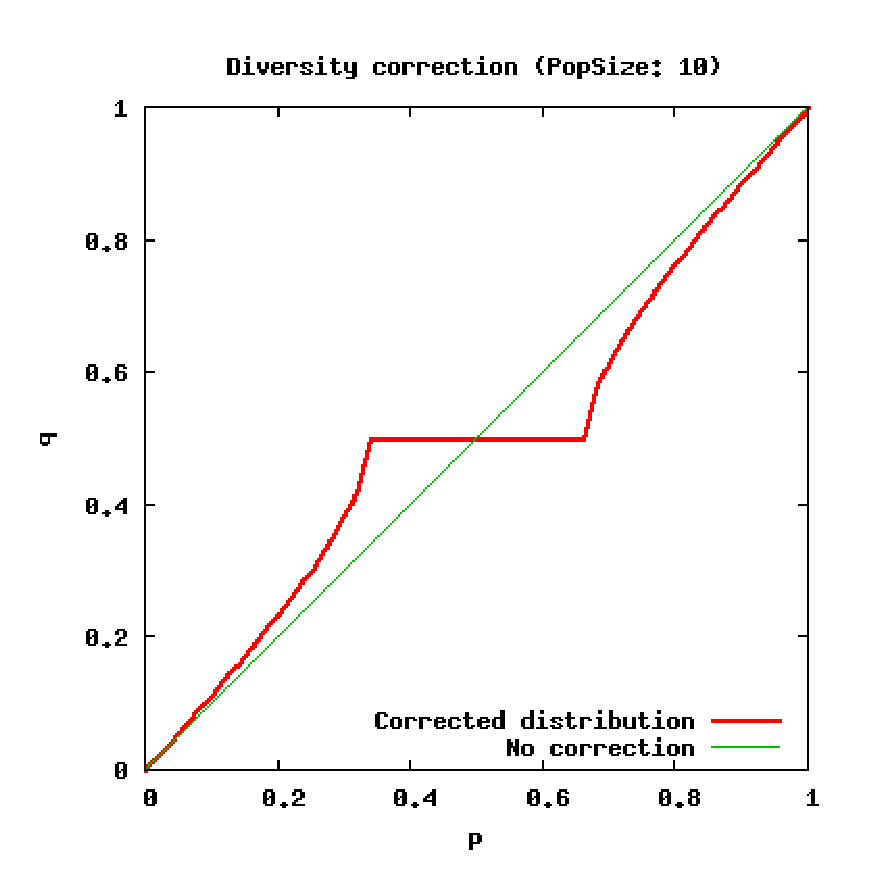
\includegraphics[scale=0.4]{graph_DC_correction.eps}
\mycaption{Correction graph for Distribution Correction}
\label{dc_correction_1}
\end{wrapfigure}


If our \(p\) is within \(p_{1}\) and \(p_{2}\)
\[
\frac{1}{2} (1 - \sqrt{1 - \frac{M(N-1)}{N(M-1)}}) < p < \frac{1}{2} (1 + \sqrt{1 - \frac{M(N-1)}{N(M-1)}})
\]
we will have to substitute with an appropriate value. As the function approaches \(0.5\) both from the top and from the bottom we will substitute with \(q = 0.5\) if our \(p\) is within those borders. In figure \ref{dc_correction_1} you can see the graph of the correction function for a population size of 10. The green line represents \(f(p) = p\), i.e. no correction takes place. The larger the population size is the smaller is the horizontal line in the middle, i.e. the substitution with \(p = 0.5\).


\newpage
\subsection{Code}
Finally we can put our results into a code (\(M = 2N\)):\\

\begin{verbatim}
if( p < (1 - sqrt( 1 - 1 / N(2*N-2) / (2*N-1) ))/2 )
    q = (1 - sqrt( 1 - (2*N-1) / (2*N-2) * 4*p*(1-p) ) )/2;
else
if( p > (1 + sqrt( 1 - (2*N-2) / (2*N-1) ))/2 )
    q = (1 + sqrt( 1 - (2*N-1) / (2*N-2) * 4*p*(1-p) ) )/2;
else
    q = 1/2;
\end{verbatim}

or for random values of population size \(M\) and sampling size \(N\):\\
         
\begin{verbatim}
if( p < (1 - sqrt( 1 - (M*(N-1)) / (N*(M-1)) ) )/2 )
    q = (1 - sqrt( 1 - (N*(M-1)) / (M*(N-1)) * 4*p*(1-p) ) )/2;
else 
if( p > (1 + sqrt( 1 - (M*(N-1)) / (N*(M-1)) ) )/2 )
    q = (1 + sqrt( 1 - (N*(M-1)) / (M*(N-1)) * 4*p*(1-p) ) )/2;
else
    q = 1/2;
\end{verbatim}

or for random values of population size \(M\) and sampling size \(N\):\\
         
\begin{verbatim}
if( p < 0.5 * (1 - sqrt( (M*(N-1)) / (N*(M-1)) ) ) )
    q = 0.5 * (1 - sqrt( (N*(M-1)) / (M*(N-1)) * 4*p*(1-p) ) );
else 
if( p > 0.5 * (1 + sqrt( (M*(N-1)) / (N*(M-1)) ) ) )
    q = 0.5 * (1 + sqrt( (N*(M-1)) / (M*(N-1)) * 4*p*(1-p) ) );
else
    q = 0.5;
\end{verbatim}

It is easy to implement the code piece within an existing application as it is problem independent (within the restrictions described above, bit-strings on a flat landscape in UMDA). The code itself has to be inserted just after determining the distribution \(p\) from the selected part of the population of the size \(N\).

\newpage

\section{Exact Distribution (ED)}

So far we have calculated that the variance loss of generating a population on basis of \(p\) randomly (i.e. with 'Random Distribution') will result in a variance loss of \(1 - \frac{1}{M}\). In order to create a new generation we originally set each value of each component of an individual of the new population to '1' with the probability of \(p\) (or to '0' with the probability of \(1-p\)). \\
A different approach is to create the new generation by distributing exactly \(p \cdot M\) '1's (or \((1-p) M\) '0's) within the array of components in the population so that the new variance is exactly \(p (1 - p)\), i.e. there is no variance loss between step III and IV. You can see that in figure~\ref{exact_distribution_1}, the methods using Exact Distribution perform better in fitness and in diversity.\\
For this method our \(p\) is calculated this way:
\[
p = \frac{k_{old}}{N}
k_{new} = \lfloor p M \rfloor = \lfloor \frac{k_{old} M}{N} \rfloor
\]

\(k_{old}\) denotes the number of '1's in the last generation, \(k_{new}\) denotes the number of '1's in the generation we are about to create. \(\lfloor p M \rfloor = \lfloor \frac{k_{old} M}{N} \rfloor\) does only apply when we do not change \(p\) through any correction method (like Laplace Correction). In the next section we will discuss how we can handle the rounding error for methods that use both a correction method for \(p\) and use Exact Distribution.

\begin{figure}[H]
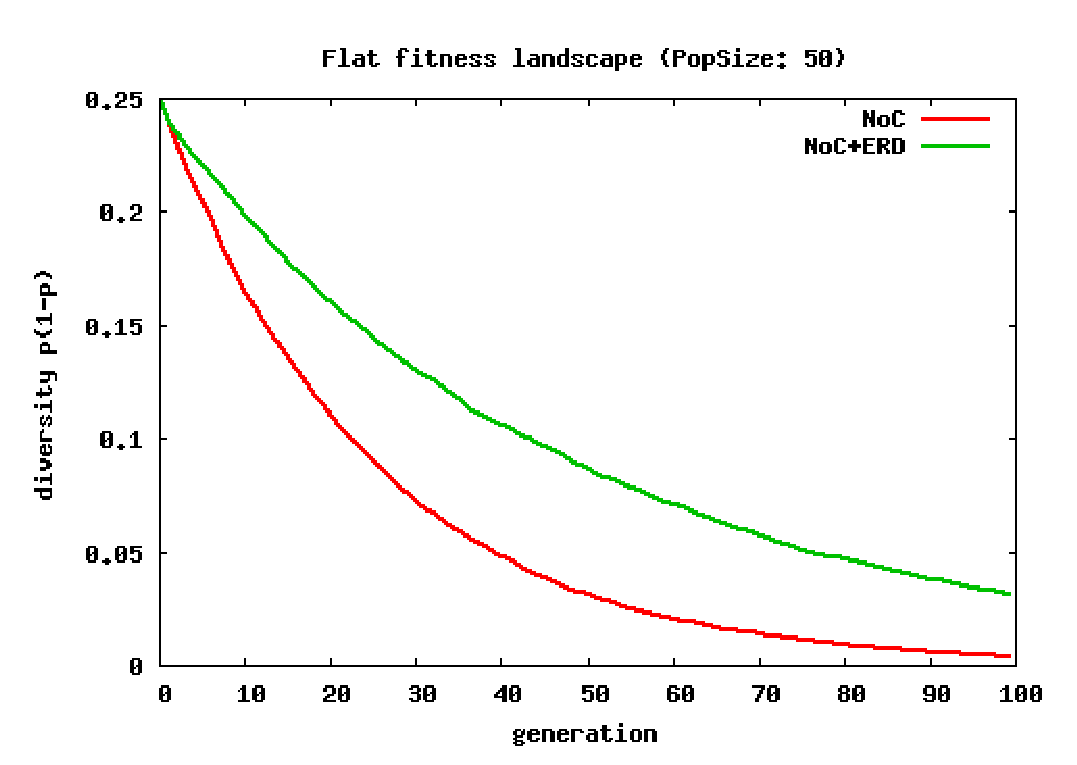
\includegraphics[scale=0.4]{graphs/graph_flat1161760821/graph_flat000_diversity.eps}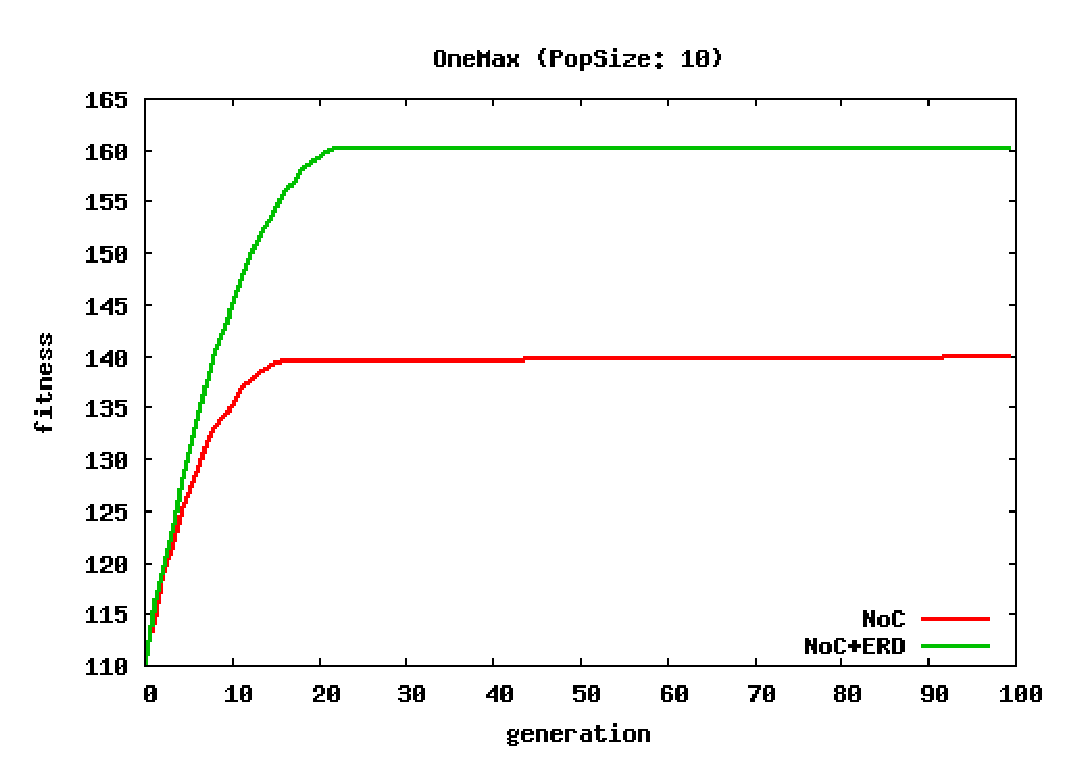
\includegraphics[scale=0.4]{graphs/graph_onemax1161765238/graph_onemax000_fitness.eps}
\mycaption{Comparison between Exact Random Distribution and Random Distribution}
\label{exact_distribution_1}
\end{figure}

\subsection{Exact Distribution Correction}

In the Chapter 4 we have discussed how to reduce the variance loss if we create the population with Random Distribution. When using an Exact Distribution the diversity loss \(d_p\) is different and we cannot use the same Diversity Correction method as before so we have to adapt the equations to the new situation. For now we will ignore the rounding error and assume that there are exactly \(p \cdot M\) '1's in the population. So we have to change in equation~(\ref{eq:probabilityk}) the probability for \(\tilde{p_{i}} = \frac{k_{i}}{M}\):

\[
\dot{P}_(\tilde{p_{i}} = \frac{k_{i}}{M}) = \left\{
\begin{array}{l l}
1 & \quad \mbox{for \(k_{i} = p_{i}M\)}\\
0 & \quad \mbox{for \(k_{i} \neq p_{i}M\)}\\
\end{array}
\right.
\]


The other equations (\ref{eq:variance1}), (\ref{eq:variance2}), (\ref{eq:variance3}), (\ref{eq:variance4}) about our variance \(v_{k_{i}}\) remain the same as they are dependent on our \(k_{i}\) anyways. Changes have to be made to equation~(\ref{eq:totalv}) because our \(P(\tilde{p_{i}} = \frac{k_{i}}{M})\) has changed. We no longer sum over all possible values of \(k\) as only (\(k = p \cdot M\)) has the probability '1' while all other values for \(k\) have the probability '0':

\begin{equation}
\dot{d}_p = \sum_{i=1}^C  v_{k_{i} = p_{i} M} P(\tilde{p_{i}} = \frac{k_{i} = p_{i}M}{M}) = 
\sum_{i=1}^C  v_{p_{i} M} \cdot 1 =\\
\sum_{i=1}^C \frac{p_{i} M^{2} - (p_{i} M)^{2}}{M^{2}} = 
\sum_{i=1}^C p_{i} (1 - p_{i})
\end{equation}


As expected we have no loss of variance from step (III) to step (IV) using Exact Random Distribution because \(\frac{\dot{d}_p}{p(1-p)} = 1\) and we get in an analogous manner the factor of variance loss from step (II) to (III) with 
\[
y = 1 - \frac{1}{N} \quad \mbox{and} \quad x = \frac{1}{1 - \frac{1}{N}} = \frac{N}{N-1}
\]
The problem is that we cannot easily insert that into equation~(\ref{eq:qpx}) and use the new distribution vector to generate the new population because we have demanded that \(p \cdot M\) (with \(p\) being the distribution vector with which we create the new generation) is a whole number. If we change the distribution vector we probably do have a rounding error which we did not include in our calculation above. We will look into that a little closer in the next chapter, for now we will accept that there is a small error in our calculation and examine if the algorithm does well in the tests anyways.\\
Inserting our \(x\) into equation~(\ref{eq:qpx}) we will get \(q(1-q) = p(1-p) \frac{N}{N-1}\) and we have

\begin{wrapfigure}{r}[0cm]{5.5cm}
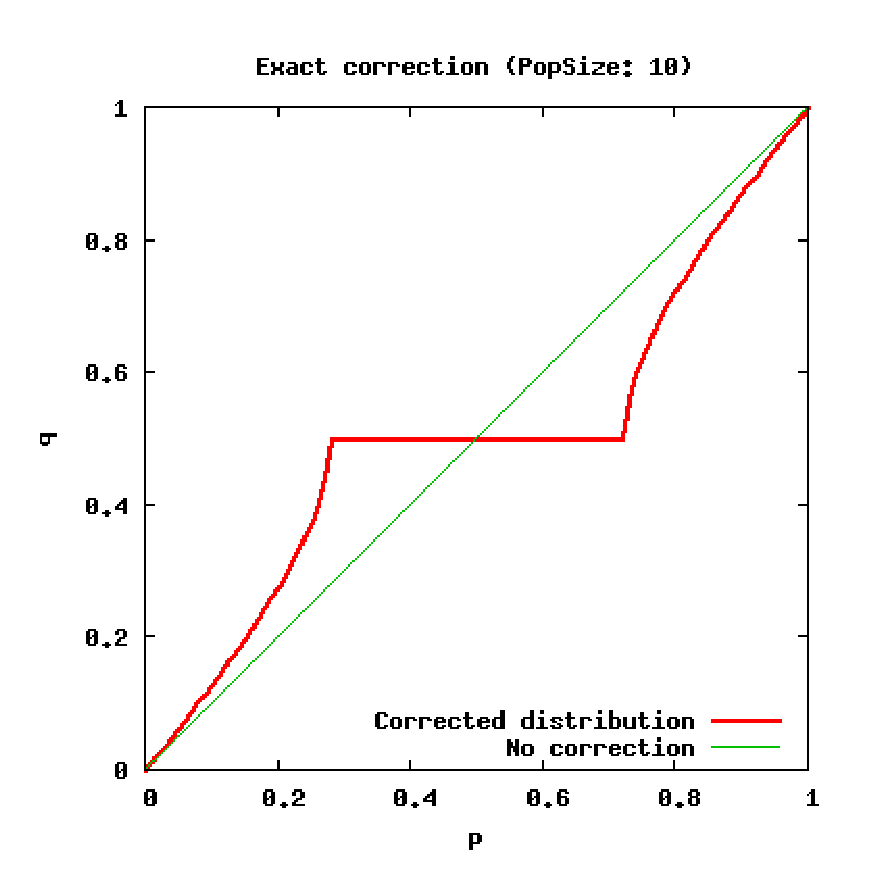
\includegraphics[scale=0.4]{graph_EC_correction.eps}
\mycaption{Correction graph for Exact Distribution Correction}
\label{ec_correction_1}
\end{wrapfigure}

\[
\dot{q}(1-\dot{q}) = p(1-p) \frac{N}{N-1} \Leftrightarrow
\]
\[
-\dot{q}^2 + \dot{q} - (-p^2 + p) \frac{N}{N-1} = 0 \Leftrightarrow
\]
\[
\dot{q}_{1/2} = \frac{1}{2} (1 \pm \sqrt{1 - 4 (-p^2 + p) \frac{N}{N-1}})
\]

For \(1 - 4 (-p^2 + p) \frac{N}{N-1} < 0\) we get a negative value in square root. The border values for p are:
\[
1 - 4 (-p^2 + p) \frac{N}{N-1} = 0 \Leftrightarrow p_{1/2} = \frac{1}{2} (1 \pm \sqrt{1 - \frac{N-1}{N}})
\]

In figure~\ref{comparison_exact_1} you can see that 'Exact Distribution Correction + Exact Random Distribution' has the slowest convergence rate but reaches the best fitness level and that it has - as expected - the lowest variance loss on a flat fitness landscape.

\begin{figure}[H]
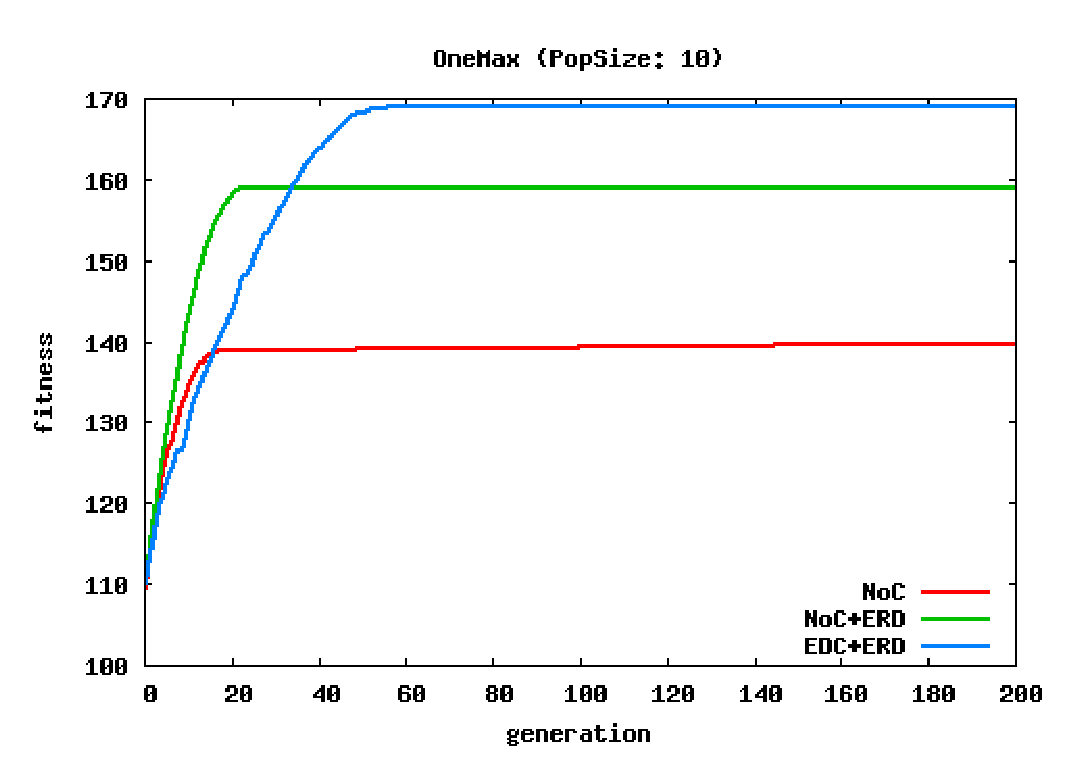
\includegraphics[scale=0.4]{graphs/graph_onemax1161768989/graph_onemax002_fitness.eps}
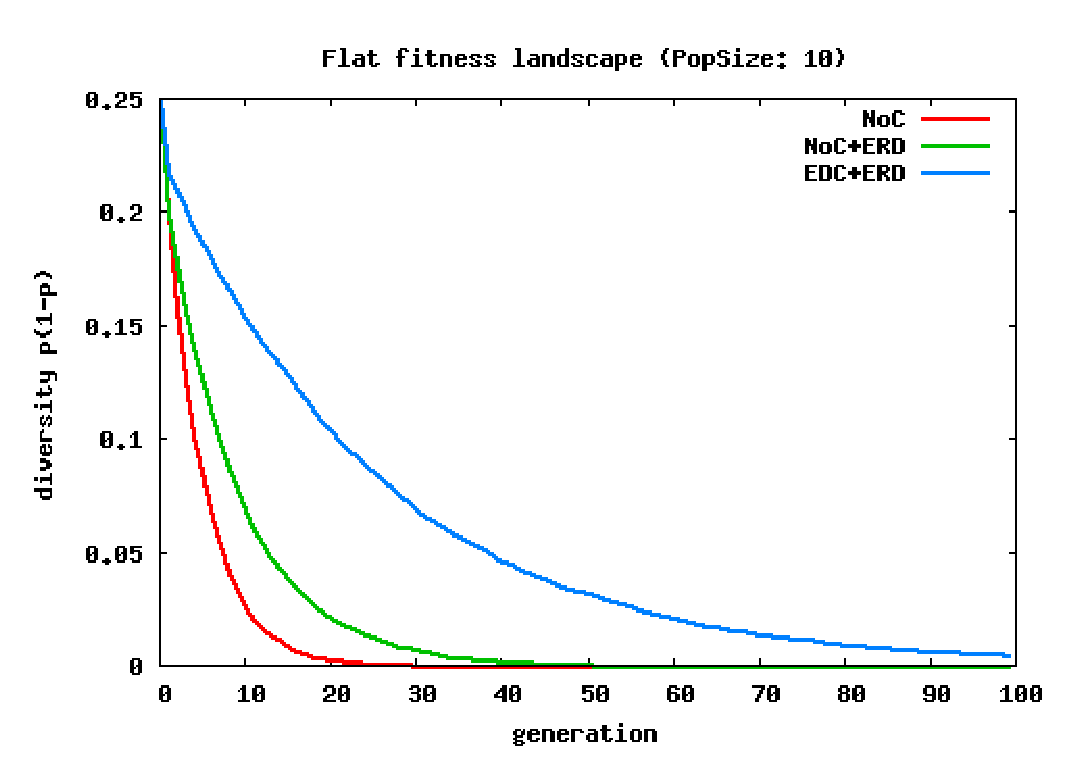
\includegraphics[scale=0.4]{graphs/graph_flat1161769173/graph_flat000_diversity.eps}
\mycaption{Exact Distribution Correction has the lowest variance loss and reaches the highest fitness level}
\label{comparison_exact_1}
\end{figure}

Compared with the Distribution Correction from last the previous chapters we can also see (figure~\ref{comparison_exact_2}) a significantly lower fitness loss on a flat fitness landscape and a better performance with the OneMax problem:

\begin{figure}[H]
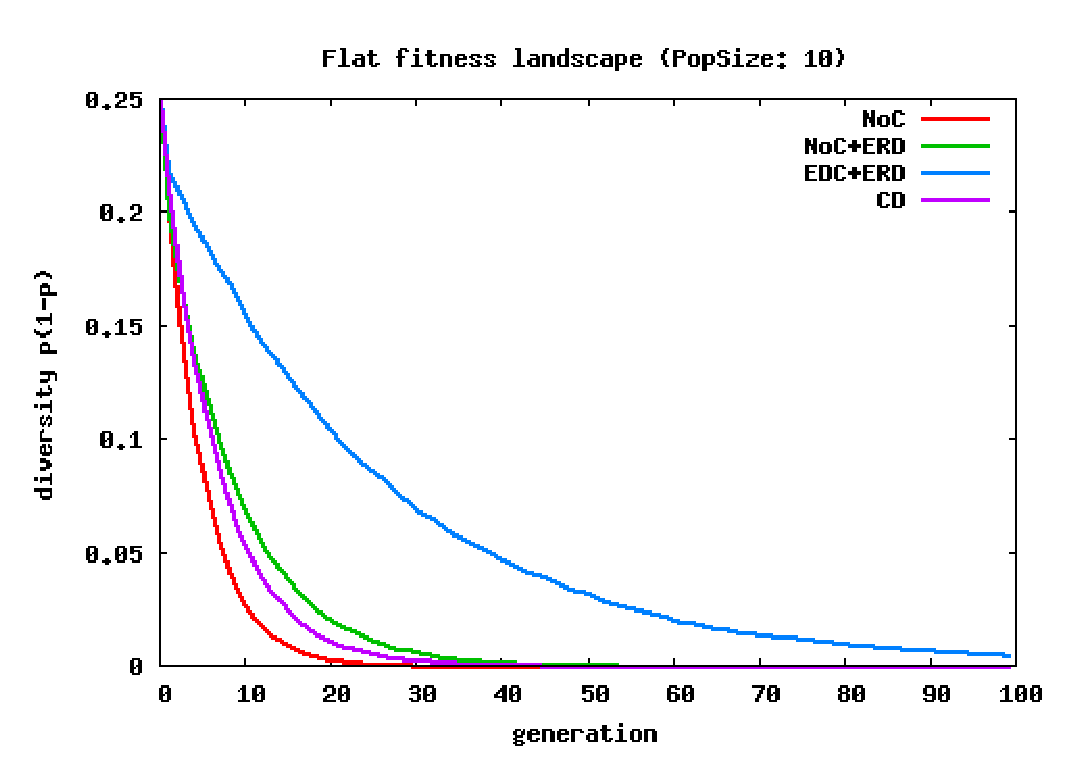
\includegraphics[scale=0.4]{graphs/graph_flat1161769606/graph_flat000_diversity.eps}
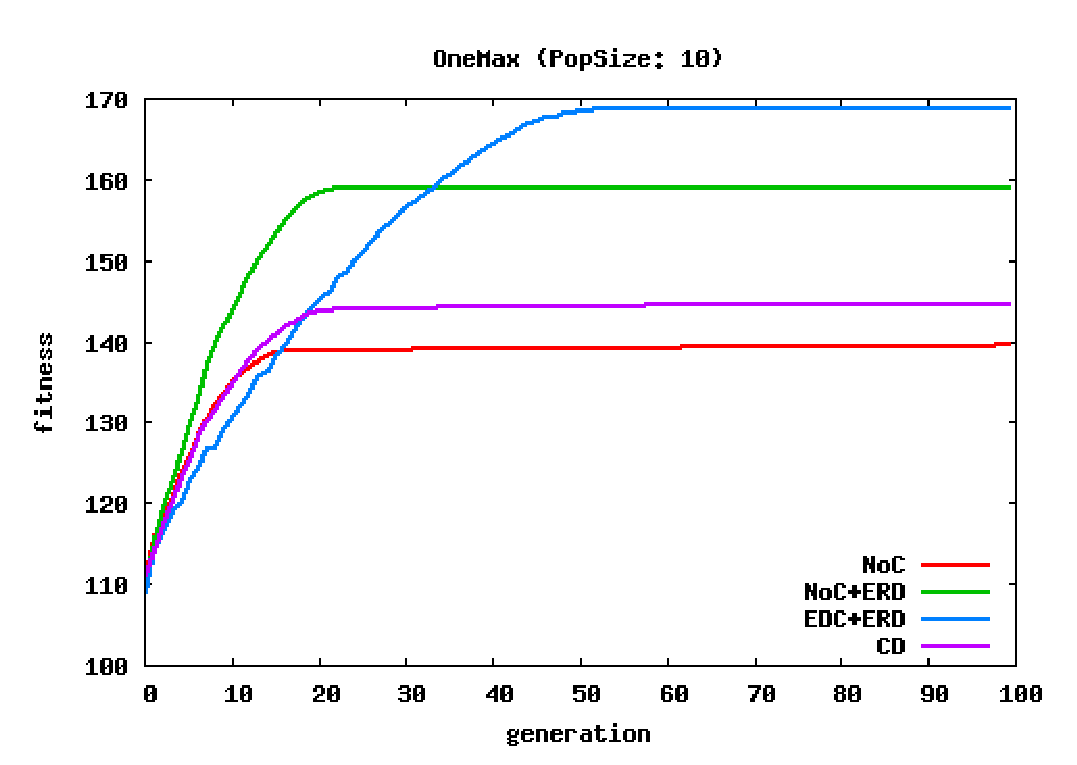
\includegraphics[scale=0.4]{graphs/graph_onemax1161769959/graph_onemax000_fitness.eps}
\mycaption{Comparison of 'Exact Distribution Correction' with 'Distribution Correction'}
\label{comparison_exact_2}
\end{figure}

\subsection{Code}
Again we can put the results into into a code. There is no difference compared to the code of Diversity Correction except that the factor inside the square root and that it is independent from \(M\):\\

\begin{verbatim}
if( p < (1 - sqrt( 1 - (N-1)/N ))/2 )
    q = (1 - sqrt( 1 - N/(N-1) * 4*p*(1-p) ) )/2;
else
if( p > (1 + sqrt( 1 - (N-1)/N ))/2 )
    q = (1 + sqrt( 1 - N/(N-1) * 4*p*(1-p) ) )/2;
else
    q = 1/2;
\end{verbatim}

\newpage
\subsection{Rounding errors}

Rounding errors are a big problem as with iterative algorithms like EDAs they will multiply over time. If an algorithm is for example biased towards '1' due to rounding it will do great in a simple OneMax test but fail miserably in a 'ZeroMax' test.\\
When we analyze this option within our framework that we have set in the last two sections we see that a rounding error occurs when \(p \cdot M\) is no whole number. When we simply calculate \(p\) by counting the number of '1's in the selected part of the population of size \(N\) such a rounding error will only occur if \(M\) is no multiple of \(N\).\\
No problem here, but this becomes an issue if we try to combine for example the {\bf Laplace correction} or the {\bf Distribution Correction} with Exact Distribution, because those methods change \(p\) before we distribute \(p \cdot M\) '1's within our population and that new \(\dot{p} \cdot M\) is not necessarily a whole number, no matter whether \(M\) is a multiple of \(N\) or not.\\
Thus, when using Exact Distribution, we can demand that \(\lfloor p \cdot M \rfloor = p \cdot M\), round the number to the nearest whole number or, depending on the remainder, randomly decide whether to add another '1' (e.g. for \(p = 0.71\) and \(M = 10\) we would distribute seven '1's and an eighth '1' with the probability of \(0.1\)). 
The drawback for the latter two methods is that the distribution no longer deserves the title 'exact' although we still get a lower variance loss.

\subsection{Real Exact Distribution Correction}

As discussed in the previous section we cannot demand that our \(p \cdot M\) is a whole number while changing the \(p\) with the Exact Distribution Correction discussed there. Using the second method mentioned in the Rounding Errors section (randomly decide whether to generate one additional '1') in equation~(\ref{eq:probabilityk}) the probability for \(\tilde{p_{i}} = \frac{k_{i}}{M}\) obviously changes as there are \(\lfloor p \cdot M \rfloor\) '1's with the probability \(1-(p \cdot M - \lfloor p \cdot M \rfloor)\) and \(\lfloor p \cdot M \rfloor+1\) '1's with the probability \(p \cdot M - \lfloor p \cdot M \rfloor\):

\[
\dot{P}_(\tilde{p_{i}} = \frac{k_{i}}{M}) = \left\{
\begin{array}{l l}
1-(p M-\lfloor p M \rfloor) & \quad \mbox{for \(k_{i} = \lfloor p_{i} M \rfloor\)}\\
p M-\lfloor p M \rfloor & \quad \mbox{for \(k_{i} = \lfloor p_{i} M \rfloor+1\)}\\
0 & \quad \mbox{else}\\
\end{array}
\right.
\]

Again, the equations about our variance \(v_{k_{i}}\) remain the same and changes have to be made to equation~(\ref{eq:totalv}) because our \(P\tilde{p_{i}} = \frac{k_{i}}{M})\) has changed and we no longer sum over all possible values of \(k\) but only two:

\[
\dot{d}_p = \sum_{i=1}^C  \sum_{k_{i}=0}^{M} v_{k_{i}} P(\tilde{p_{i}} = \frac{k_{i}}{M}) = 
\]
\[
            \sum_{i=1}^C                     v_{k_{i} = \lfloor p_{i} M \rfloor}   P(\tilde{p_{i}} = \frac{k_{i} = \lfloor p_{i} M \rfloor}{M}) +
                                             v_{k_{i} = \lfloor p_{i} M \rfloor+1} P(\tilde{p_{i}} = \frac{k_{i} = \lfloor p_{i} M \rfloor+1}{M}) =
\]
\[
            \sum_{i=1}^C                     v_{\lfloor p_{i} M \rfloor}   (1-(p M-\lfloor p M \rfloor))
                                             v_{\lfloor p_{i} M \rfloor+1}    (p M-\lfloor p M \rfloor) =
\]
\[
	    \sum_{i=1}^C  \frac{\lfloor p_{i} M \rfloor M - \lfloor p_{i} M \rfloor^{2}}{M^{2}} (1-(p M-\lfloor p M \rfloor)) +
			  \frac{(\lfloor p_{i} M \rfloor+1) M - (\lfloor p_{i} M \rfloor+1)^{2}}{M^{2}} (p M-\lfloor p M \rfloor) =
\]
\[
	    \sum_{i=1}^C  \frac{
				(\lfloor p_{i} M \rfloor)^2 - 2 \lfloor p_{i} M \rfloor p M + p M^{2} - p M + \lfloor p M \rfloor}
				{M^{2}
			       }
\]

Our variance loss is as before \(\frac{\dot{d}_p}{p (1-p)}\) which unfortunately cannot simplified any further and therefore is dependent on \(p\). With equation~(\ref{eq:y}) we have 
\[
y = \frac{1 - \frac{1}{N}}{\frac{\dot{d}_p}{p (1-p)}} \mbox{\quad and \quad} x = \frac{1}{y} = \frac{\frac{\dot{d}_p}{p (1-p)}}{1 - \frac{1}{N}}
\]

The problem is that we cannot easily insert that into equation~(\ref{eq:qpx}) as in this case our \(x\) depends on the distribution vector \(p\) with which we create the new population. This is a problem because the creation of our new population (Step III) happens of course {\emph after} the correction of \(p\). So we really have to make \(x\) dependent on the distribution vector \(\dot{q}\):

\[
\dot{q}(1-\dot{q}) = p(1-p) x_{\dot{q}}
\]
This is kind of difficult to solve for \(\dot{q}\) and probably has to be solved numerically. On the one hand this 'corrected' correction would further increase the effectiveness of the erroneous 'Exact Distribution Correction' discussed earlier while on the other hand it would cost more calculation time. Tests have to be made to determine if it is worth it.

\newpage
\section{General test configuration}

\subsection{Graph drawing}

The graphs were created with the help of gnuplot 4.0 and g++ 4.0 (gnu C++), the actual program will be available with a later version of this paper on CD-ROM.\\
TODO
Because all algorithms are based on random numbers 50 separate runs were made for each parameter setting and algorithm. The data then is averaged and drawn as a graph. Normally this would result in oscillating fitness graphs as shown for example in figure (\ref{oscillating_1}). The oscillation does not bear any additional information so for the sake of clarity only the best average result that was found until that point is drawn, i.e. the graphs always have a non-negative gradient.

\begin{figure}[H]
\hspace{-0.5in}
\includegraphics[scale=0.5]{graphs/graph_onemax1161026602/graph_onemax000_fitness.eps}
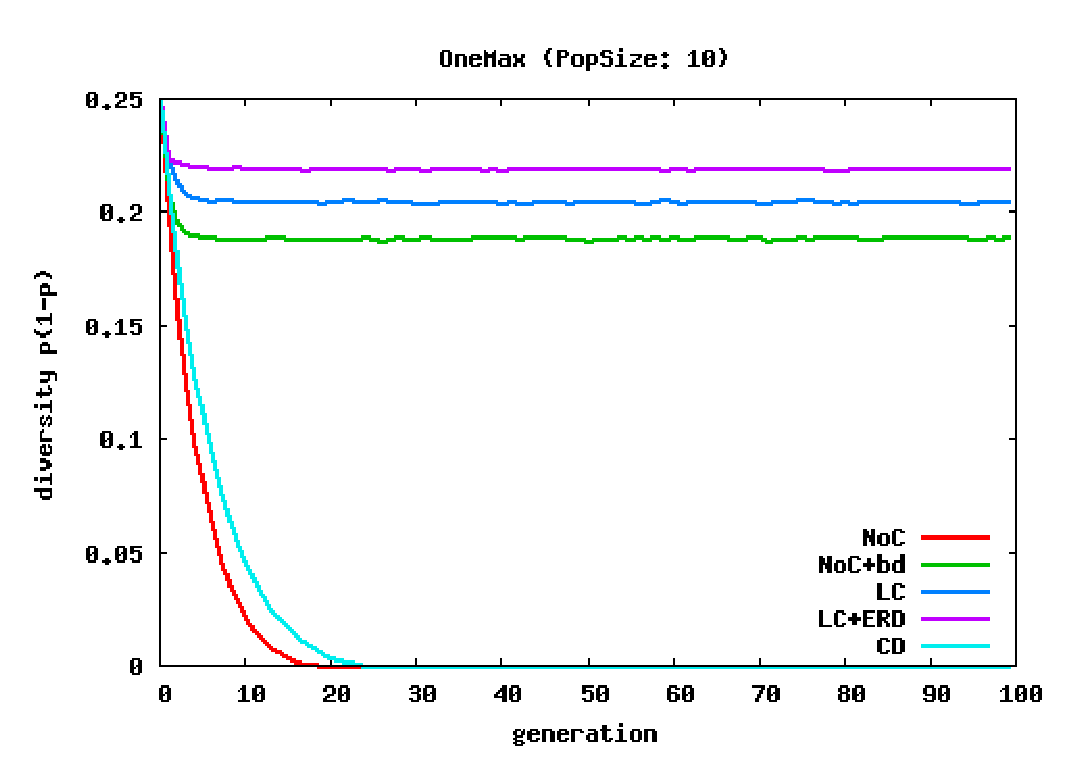
\includegraphics[scale=0.5]{graphs/graph_onemax1161026602/graph_onemax000_diversity.eps}
\mycaption{Oscillating fitness graphs}
\label{oscillating_1}
\end{figure}

In figure (\ref{oscillating_1}) you can also see that {\bf Corrected Distribution (CD)} and {\bf No Correction (NC)} do not oscillate. This is simply because their variance dropped practically to \(0\) after a few generations, i.e. no component will change anymore.\\


\subsection{Population size}

Depending on the problem type, problem size and algorithm different population sizes ranging from 10 to 100 were tested. Also for each single configuration several different population sizes were tested because the convergence speed differ between the methods. Larger populations automatically result in more diversity and less diversity loss in each generation.

\subsection{Selection size}

For problem types that do not use a flat fitness landscape we are interested in their fitness. We usually select the top 50\% from the population in order to calculate the distribution vector \(p\). Higher selection rates will reduce the convergence speed because we are including below average solutions in \(p\) while lower selection rates will significantly increase the diversity loss. If the convergence speed is reduced the method will have difficulties to reach or maintain good solutions either because the diversity dropped already to zero or (with Boundary Check or Laplace Correction) the high diversity holds back good solutions from spreading through the population. 

\begin{figure}[H]
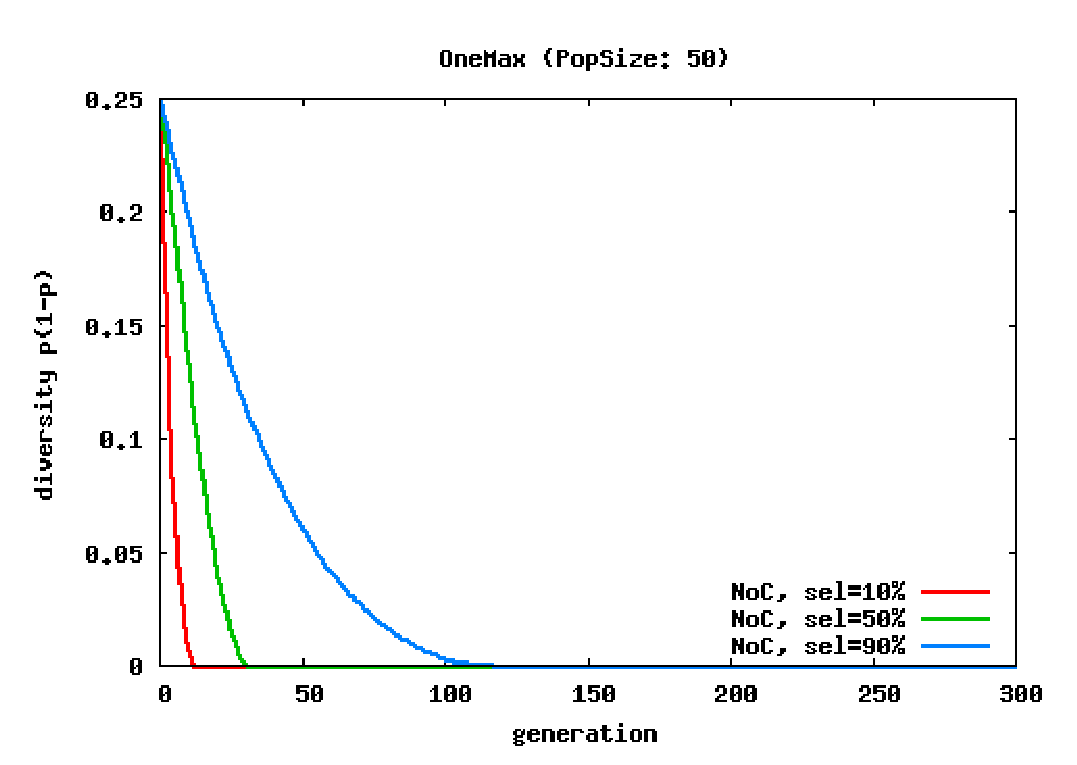
\includegraphics[scale=0.4]{graphs/graph_onemax1162139150/graph_onemax000_diversity.eps}
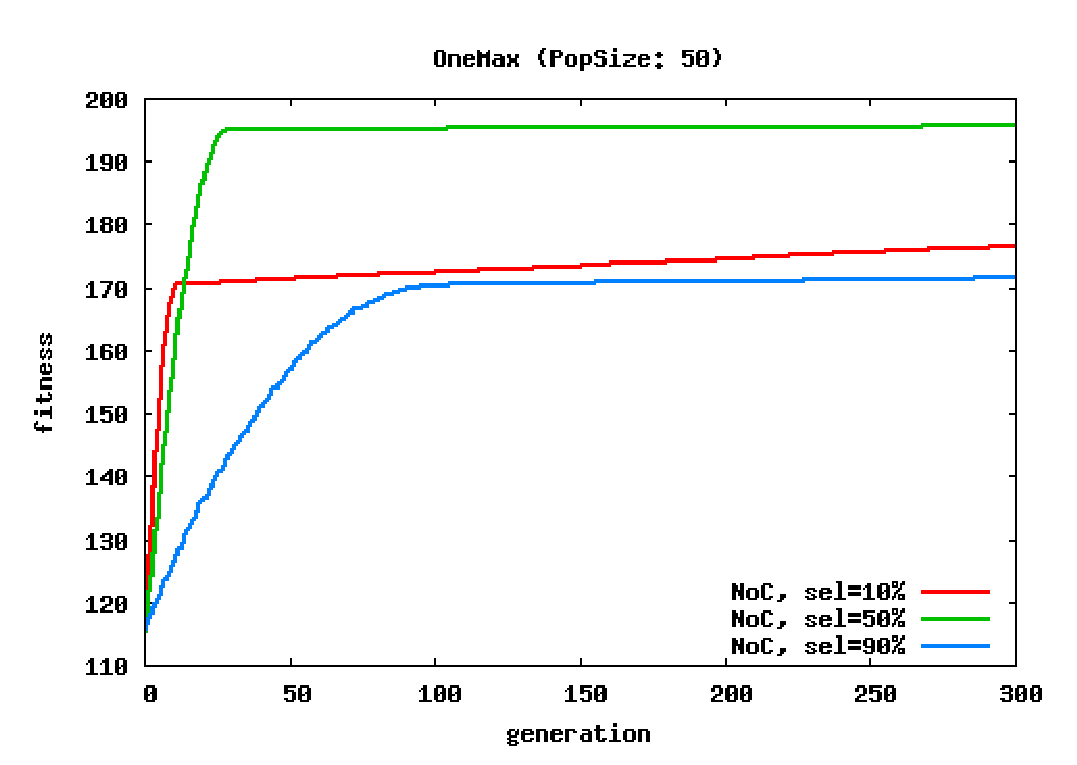
\includegraphics[scale=0.4]{graphs/graph_onemax1162139150/graph_onemax000_fitness.eps}
\mycaption{Different selection sizes}
\label{selectionsize}
\end{figure}

\newpage
\subsection{Problem types}

\subsubsection{Flat fitness landscape}

In this test we examine the behaviour of the algorithms in terms of their {\emph diversity} with varying parameters on a flat fitness landscape. It is basically a 'needle in a haystack' problem where the needle is not found within the 200 generations, i.e. all solutions have the same fitness. The problem size is a bit-string with length 10, i.e. we have 10 components.\\
The additional graph, '1 - 1/N loss / generation', denotes the theoretical loss of diversity according to \cite{Shapiro}.

\subsubsection{OneMax problem}

\begin{wrapfigure}{r}[0cm]{6.5cm}
\vspace{-0.7in}
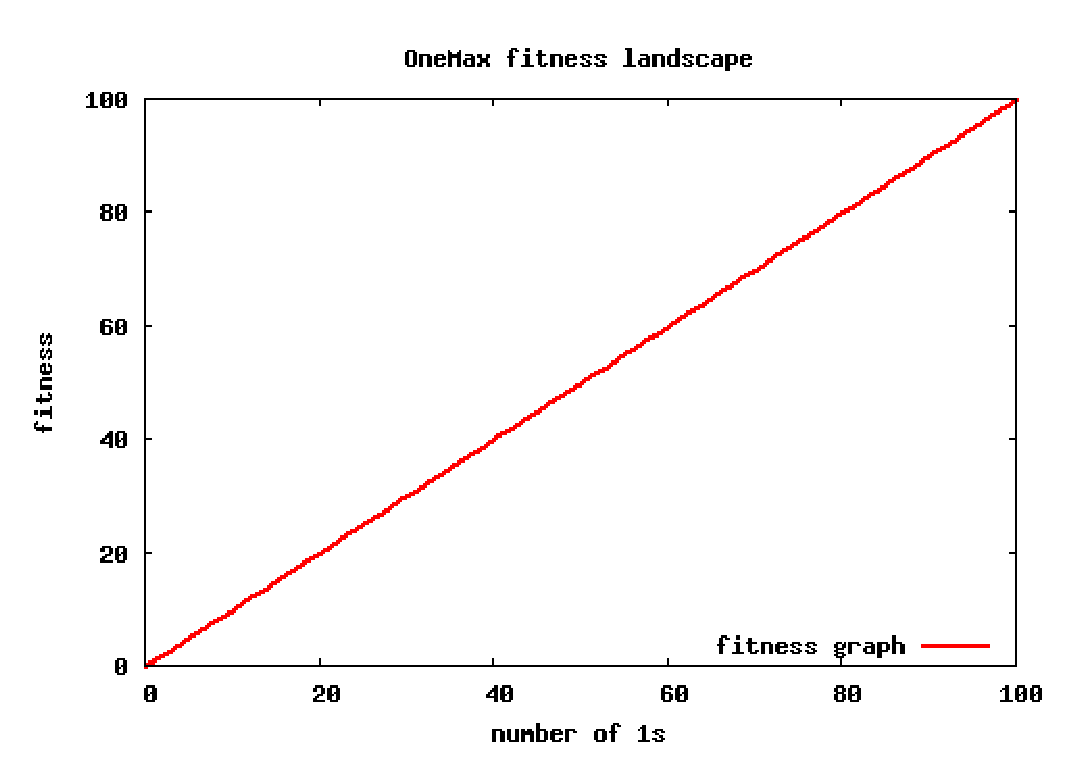
\includegraphics[scale=0.4]{graph_onemax_fitness_landscape.eps}
\mycaption{Fitness Landscape of OneMax}
\label{fitness_landscape_onemax}
\end{wrapfigure}
In this test we examine the behaviour of the algorithms in terms of their {\emph fitness} with varying parameters with the problem OneMax. The goal is to find the string '111\dots', each '1' in a component of an individual gets rewarded by one fitness point. This is also the the main difference to a flat fitness landscape, when selecting individuals for a new generation we do not randomly take \(N\) individuals and calculate our distribution vector \(p\) but we sort all individuals by their fitness and only select the top 50\%.\\
 While the OneMax problem does not represent a problem with a real flat fitness landscape (thus the theory we discussed earlier does not apply here), a local flat fitness landscape can occur if the variance drops and/or the fitness values of the population are very similar (e.g. 010, 100, 001).\\
In our test the problem size ranges from 100 to 500 depending on the convergence speed of the functions that we will examine.\\



\subsubsection{Plateau Problem}

It is basically a OneMax problem with the difference that in a solution three neighbouring bits have to be '1' in order to get one fitness point. E.g. 100.110 would give 0 fitness points while 111.110 or 000.111 would give 1 fitness point. The problem size is of course a multiple of 3, usually 300.

%\begin{figure}[H]
%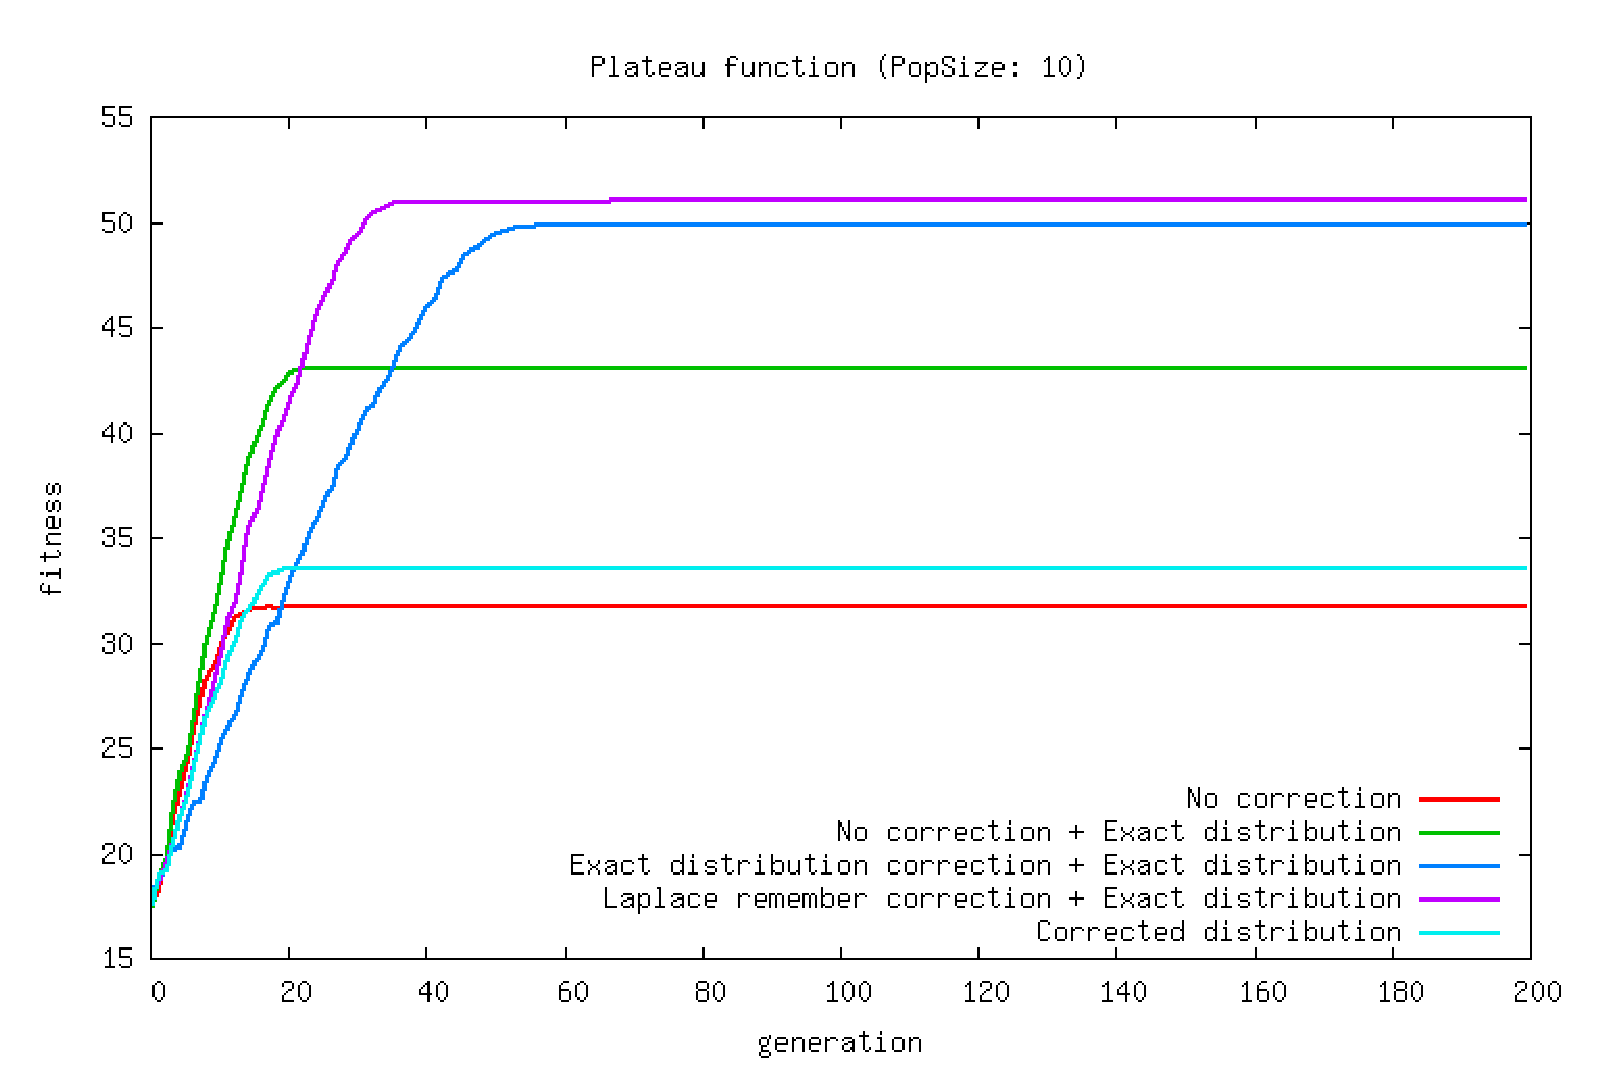
\includegraphics[scale=0.35]{graph_plateau000_fitness.eps}
%\mycaption{Fitness landscape of OneMax with two peaks}
%\label{fitness_landscape_onemax2}
%\end{figure}
%\begin{figure}[H]
%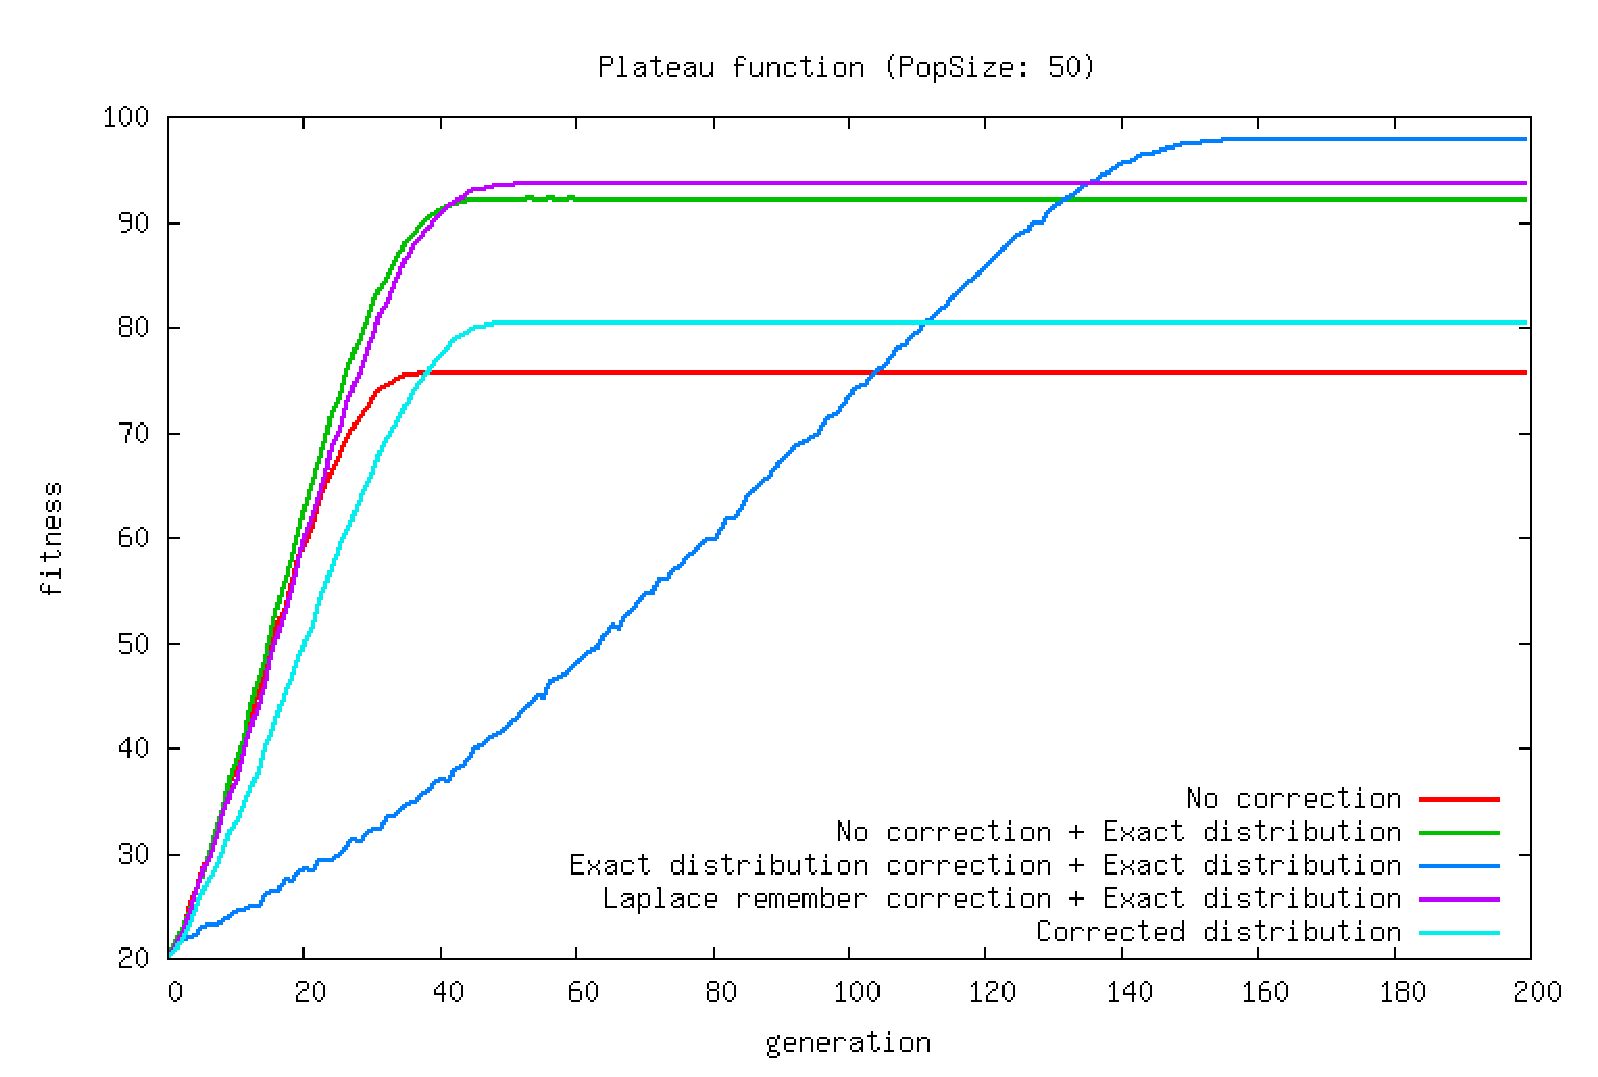
\includegraphics[scale=0.35]{graph_plateau001_fitness.eps}
%\mycaption{Fitness landscape of OneMax with two peaks}
%\label{fitness_landscape_onemax2}
%\end{figure}
% TODO
%Remember Laplace Exact Distribution does usually good for small populations and Exact Distribution + Exact Correction has again a low convergence rate but the best fitness with larger populations.

\newpage
%TODO evtl wieder raus
\subsubsection{TwoPeak problem}
\begin{wrapfigure}{r}[0cm]{6.5cm}
\vspace{-0.7in}
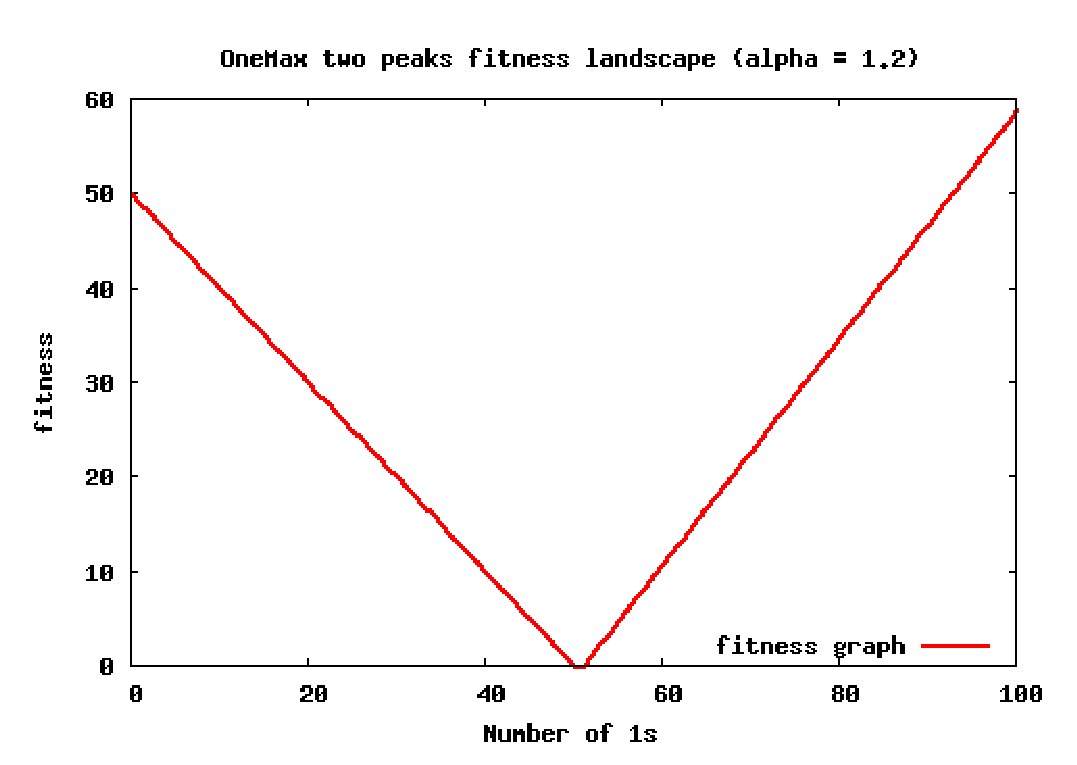
\includegraphics[scale=0.4]{graph_onemax2_fitness_landscape.eps}
\mycaption{Fitness landscape of TwoPeak}
\label{twopeak_fitness_landscape_onemax2}
\end{wrapfigure}

Similar to the OneMax problem we do count the number of equal values but not only '1's but '0's, too. There are two parameters, one defines the center where we switch from counting '0's to counting '1's and one is a factor which determines how much more (or less) worth is a '1' compared to a '0'.


%%6 different algorithms were tested: ?? TODO


\subsubsection{Leading-1s problem}

In the Leading-1s problem the fitness is calculated by counting the number of leading '1's. This implies that contrary to OneMax the bit-position is important and the bits are connected, i.e. component \(i\)'s fitness depends on all components \(j\) with \(0 < j < i\). This is more difficult to handle for UMDA's discussed in this paper.\\
For this problem keeping correct solutions on lower bit-positions is very important, i.e. lower bit-positions contribute to the total fitness more than higher bit-positions. Any algorithm that keeps up a high diversity in positions that already have the correct value will have a significantly lower fitness.

\subsubsection{NK Landscape}

From \cite{NKLandscape}:

,,An NK landscape is a real-valued function defined on the set of binary \(n\)-tuples, \(\{0,1\}^{n}\), which is of the form

\begin{equation}
f (x_1, x_2, \dots, x_n) = \sum_{i=1}^{n} f_{i} (x_i, \prod (x_i))
\end{equation}

It is a summation of local fitness functions \(f_{i}\)'s, where each \(f_{i}\) depends on its main variable \(x_{i}\) and the variables in the neighborhood of \(x_{i}\). Here the neighborhood \(\prod (x_i)\) is a subset of the set \(\{x_{1}, x_{2}, \dots, x_{n}\} \\ \{x_{i}\}\) and its size \(|\prod_{k}(x_{i})|\) is \(k\). There are two ways to choose the variables in the neighborhood \(\prod (x_{i})\), adjacent neighborhood and random neighborhood. In the NK models with adjacent neighborhood, \(\prod(x_{i})\) consists of the closest \(k\) variables (with a certain to-break) to the main variable \(x_{i}\) with respect to the indices modulo \(n\). In the NK models with random neighborhood, \(\prod(x_{i})\) is composed of the \(k\) variables chosen uniformly at random from \(\{x_{1}, x_{2}, \dots, x_{n}\}\\\{x_{i}\}\). Local fitness functions are constructed independently of each other. For each local fitness function, a random value from a probability distribution is assigned for each input.''\\

We will use a similar implementation as \cite{MitchelPotter}, with 'Random(\(x\))' denoting a function that maps \(x\) to a predefined random value.
\[
f_{i} = \frac{\mbox{Random}(2^{k})}{2^{k}}
\]

That means that each bit-pattern at each position has an own random fitness value. If a new individual is created with a similar pattern, it gets the same fitness for this pattern. For \(k = 0\) we would get a similar function as OneMax as there are only two possible values for \(f_{i}\), i.e. we are counting '1's (or '0's). For \(k = n\) we would also get a similar function as OneMax, but with different fitness values depending on the bit position. For large values of \(k\) this means that a large portion of memory is needed at the beginning (e.g. 4 GB for \(k = 32\)) so for the implementation we will use a hashtable.\\

\subsubsection{Rucksack problem}

This problem is about putting variable number of objects of variable size in a 'rucksack'. The more size of the rucksack is used the higher is the fitness. If the total size of the objects is greater than the size of the rucksack the fitness is zero.
The main issue with UMDA is how to represent the selection of objects with a binary string. I will use the implementation of \cite{rucksack}:
TODO

\newpage

\section{Additional methods}

\subsection{Boundary Check (BD)}
\begin{wrapfigure}{r}[0cm]{5.5cm}
\vspace{-0.7in}
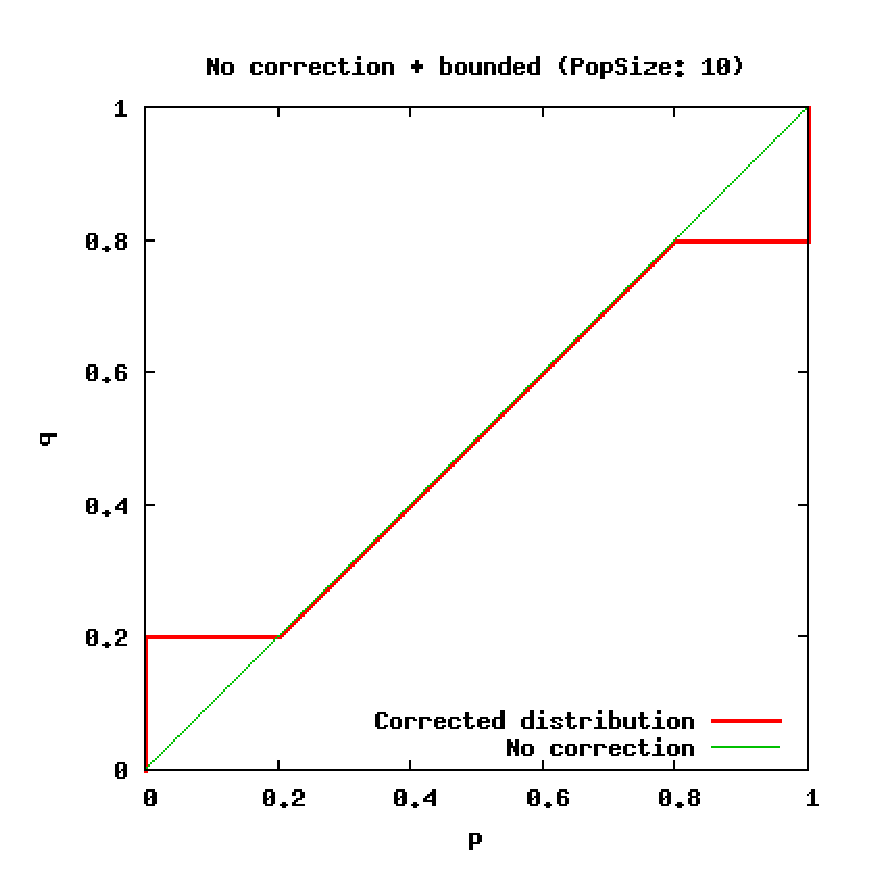
\includegraphics[scale=0.4]{graph_NC_BD_correction.eps}
\mycaption{Correction graph for Boundary Check}
\label{bd_correction_1}
\end{wrapfigure}

Another option is called {\bf bounded}. If it is set the boundaries of the final \(p\) are checked. In the case \(p\) gets above \(1 - \beta\) or below \(\beta\) it is corrected to these boundaries:

\[
p = \left\{
\begin{array}{l l}
\beta & \quad \mbox{for \(p < \beta\)}\\
1 - \beta & \quad \mbox{for \(p > 1 - \beta\)}\\
p & \quad \mbox{else}\\
\end{array}
\right.
\]

If \(\beta\) is too large the function will have problems preserving the solution. For example in the case of a OneMax problem in a situation where we have found 99 of 100 correct '1's we have to hope that none of the 99 positions will switch back to a '0' in order to find 100 '1's. 
The fitness level where a method with boundary check is expected to converge depends on all the parameters: the problem size, the population size, the problem type and the correction type. Thu
TODO



%It is clear that \(\beta\) should not be too large


%depends on the population size \(M\)?

%TODO, nicht 1/M sondern 1/alpha!

\begin{figure}[H]
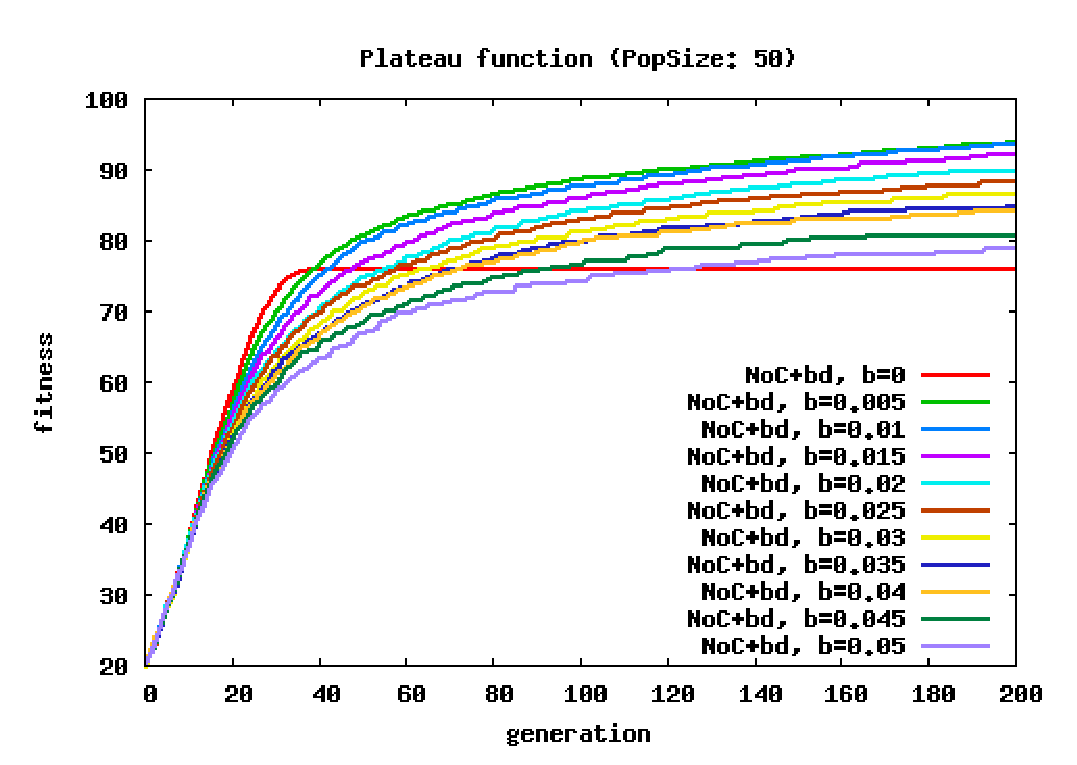
\includegraphics[scale=0.5]{graph_bounded_plateau_fitness1.eps}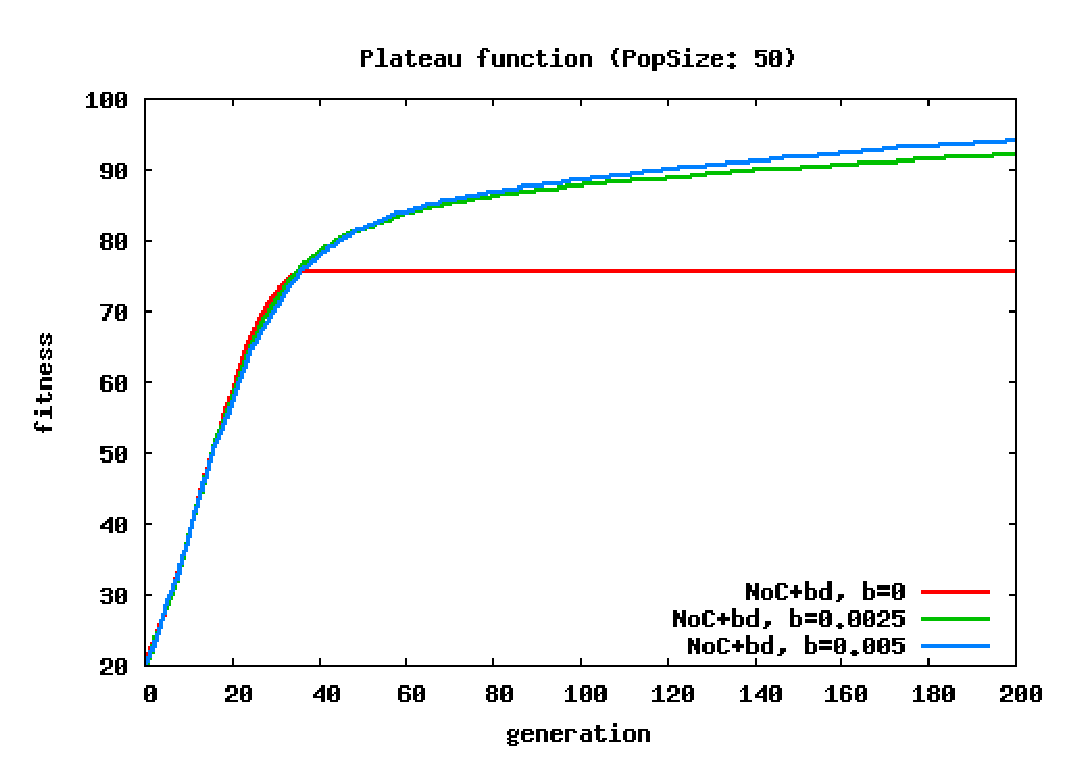
\includegraphics[scale=0.5]{graph_bounded_plateau_fitness2.eps}
\mycaption{Different values for \(\beta\), optimum at about 0.005 in this case}
\label{plateau_bounded_fitness_1}
\end{figure}

This is only useful for some of the correction algorithms that will stuck when reaching values near 0 or 1 for \(p\), i.e. if the selected part of the population contains only '0's or '1's in any component and the algorithm calculated \(p = 0.0\) or \(p = 1.0\). The boundary check theoretically ensures that any algorithm will find the optimal solution \emph{eventually} while reducing the convergence speed because values that are already determined to be optimal can be changed. In practice this is of not much use if it is the only method to prevent diversity loss but it might increase the effectiveness of some of the algorithms if the algorithm is allowed to run a very long time, see section {\bf Tests} for a comparison. Generally speaking adding the bounded option to an algorithm will reduce its convergence speed significantly but will catch up and even surpass the original algorithm several generations later depending on the parameters and the problem. TODO kuerzen


When combining Boundary Check with any of the Correction algorithms we will face the same problem as discussed with Exact Distribution. When we change our \(p\) we will also have to adapt the Correction methods. This probably have to researched TODO
An issue which will not be discussed here is that when using boundary check, our diversity will change and we would need to adapt our correction formulas accordingly if we want to use them in connection with boundary check. TODO

You can see here that with boundary check the diversity is held at a constant level. For each component there is always at least a chance of \(\frac{1}{M}\) to switch between '0' and '1'. On the one side this has the positive effect that theoretically the optimal solution will be found. On the other hand single components that already contain an optimal value can switch back to the wrong value. TODO

%TODO Vergleiche innerhalb von Gruppen, also No correction No correction+bounded, diversity correction mit diversity correction+bounded etc.

%\begin{figure}[H]
%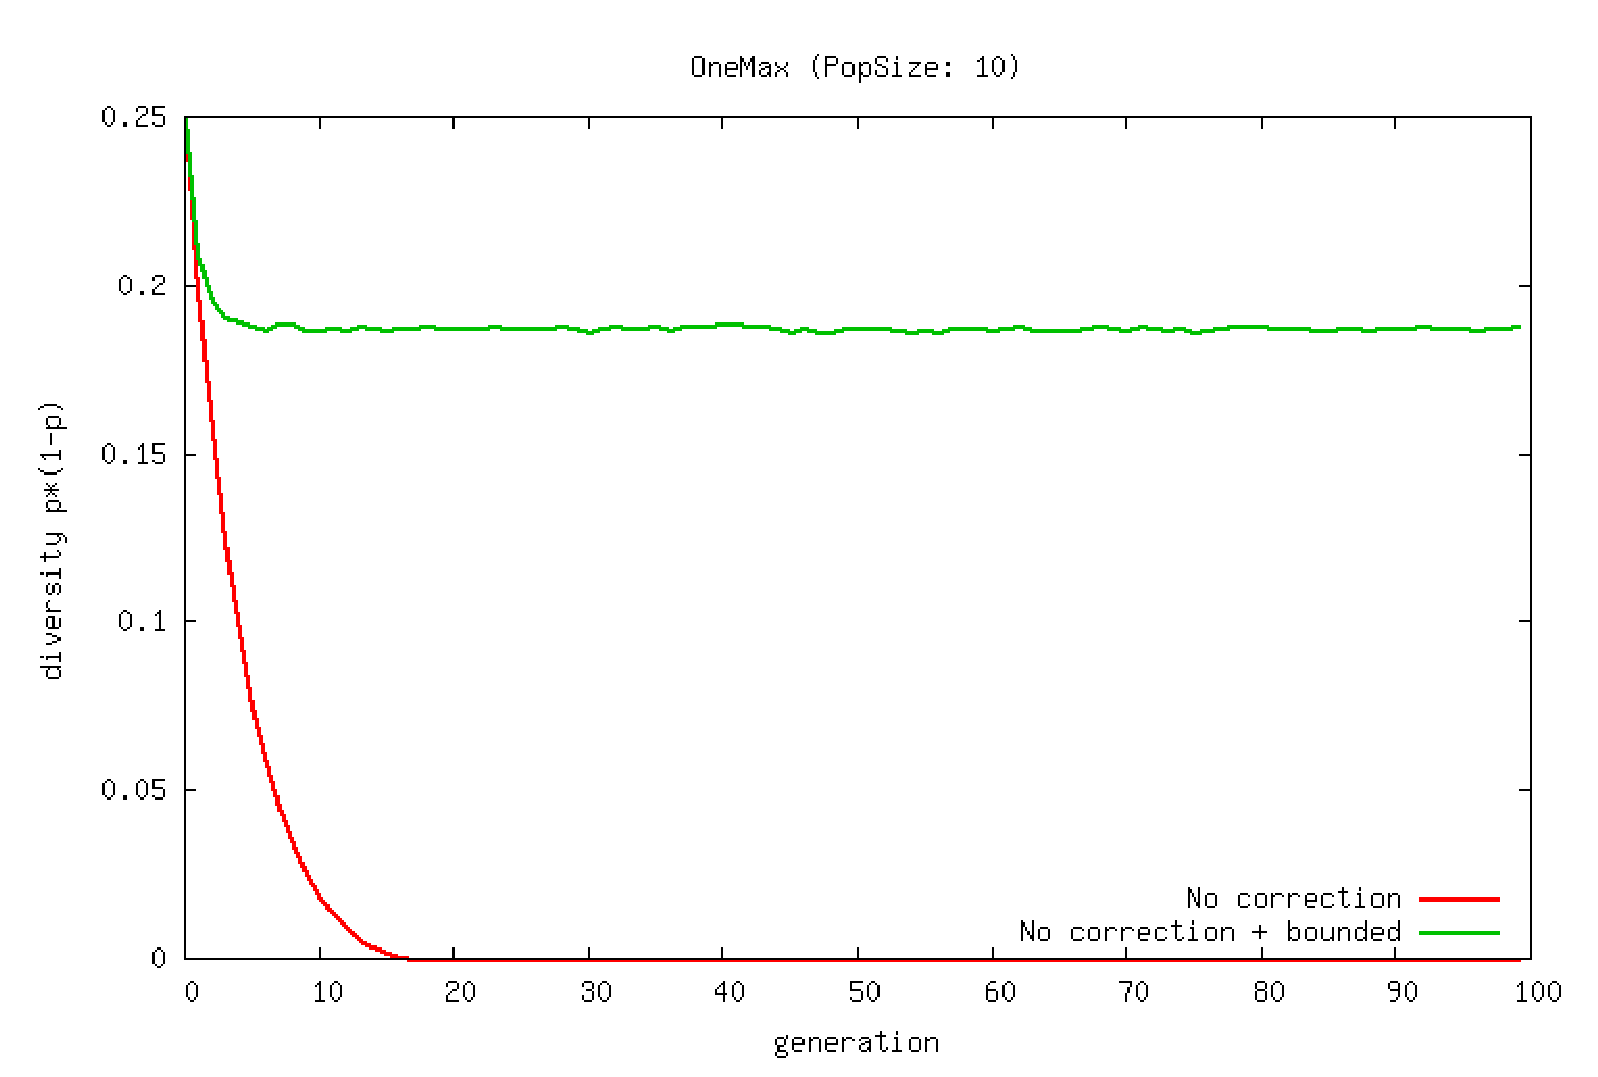
\includegraphics[scale=0.35]{graph_onemax_no_correction_bounded_diversity0.eps}
%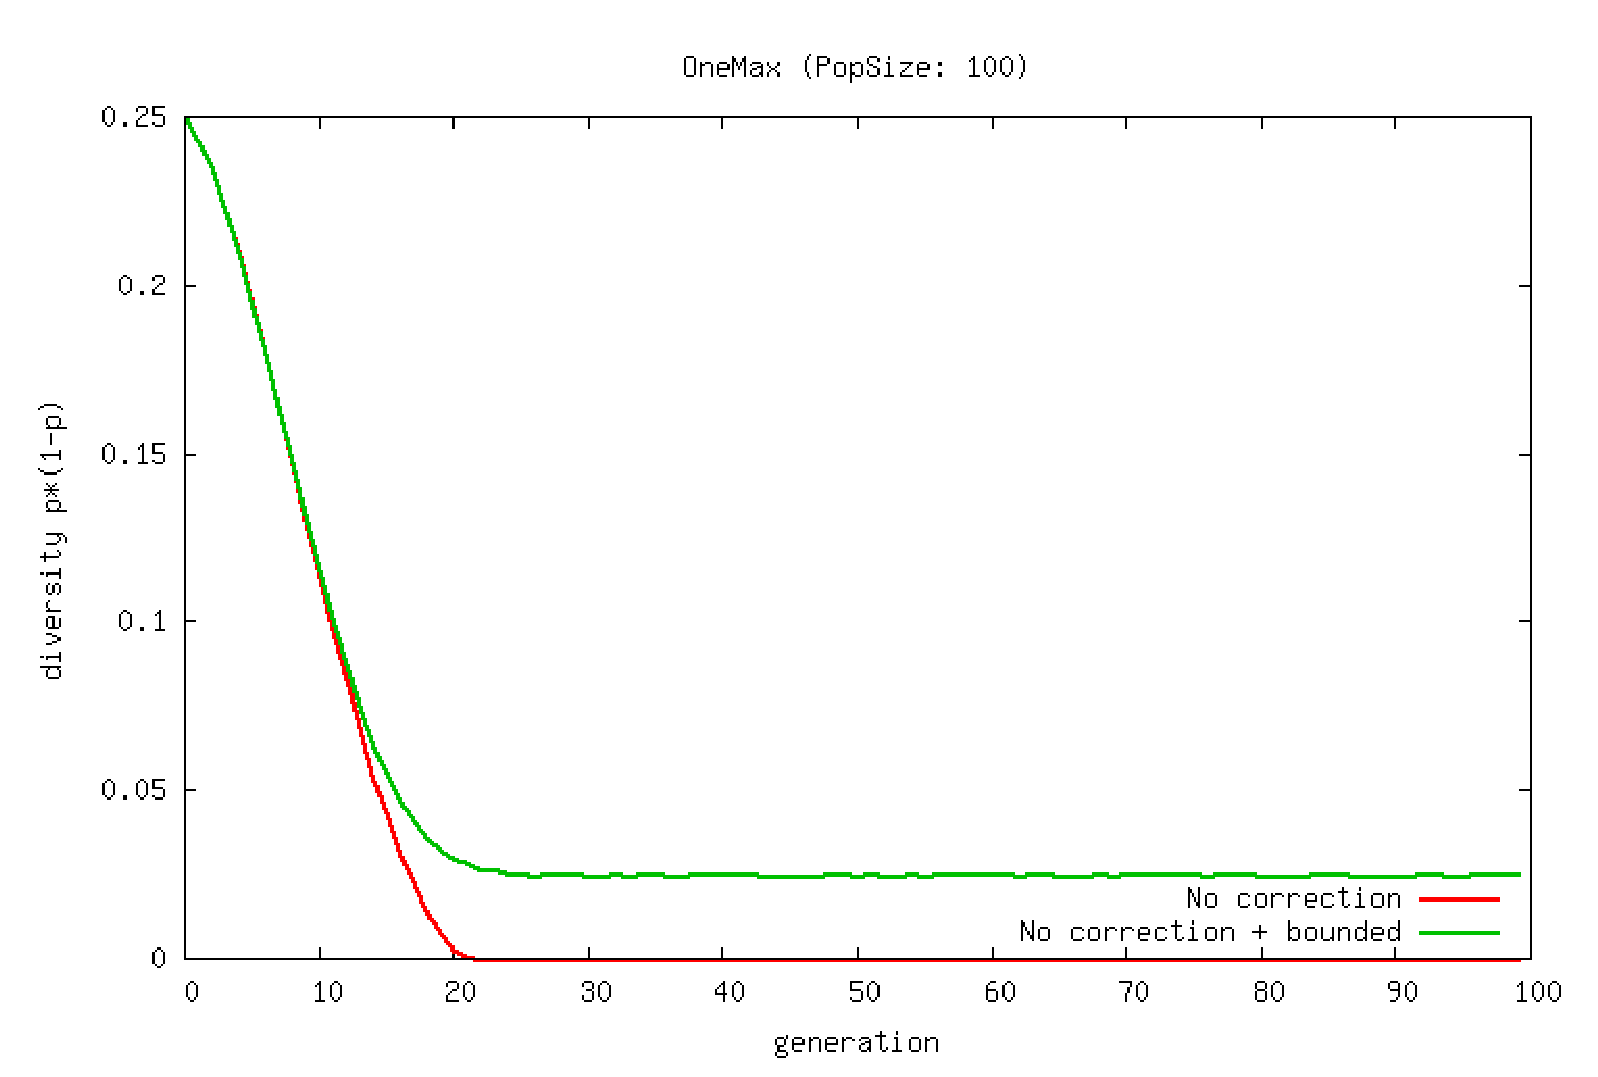
\includegraphics[scale=0.35]{graph_onemax_no_correction_bounded_diversity1.eps}
%\mycaption{With boundary check the diversity is held at a constant level}
%\label{bounded_1}
%\end{figure}
%TODO 


%For onemax we clearly see that these two opposite effects let the function converge at a lower level:

%TODO While it has a chance to find a better solution (in contrary to the method without correction) it has trouble keeping up the correct values that were found so far.

%TODO With higher population sizes this effect vanishes as \(\frac{1}{M}\) becomes smaller.

%\begin{figure}[H]
%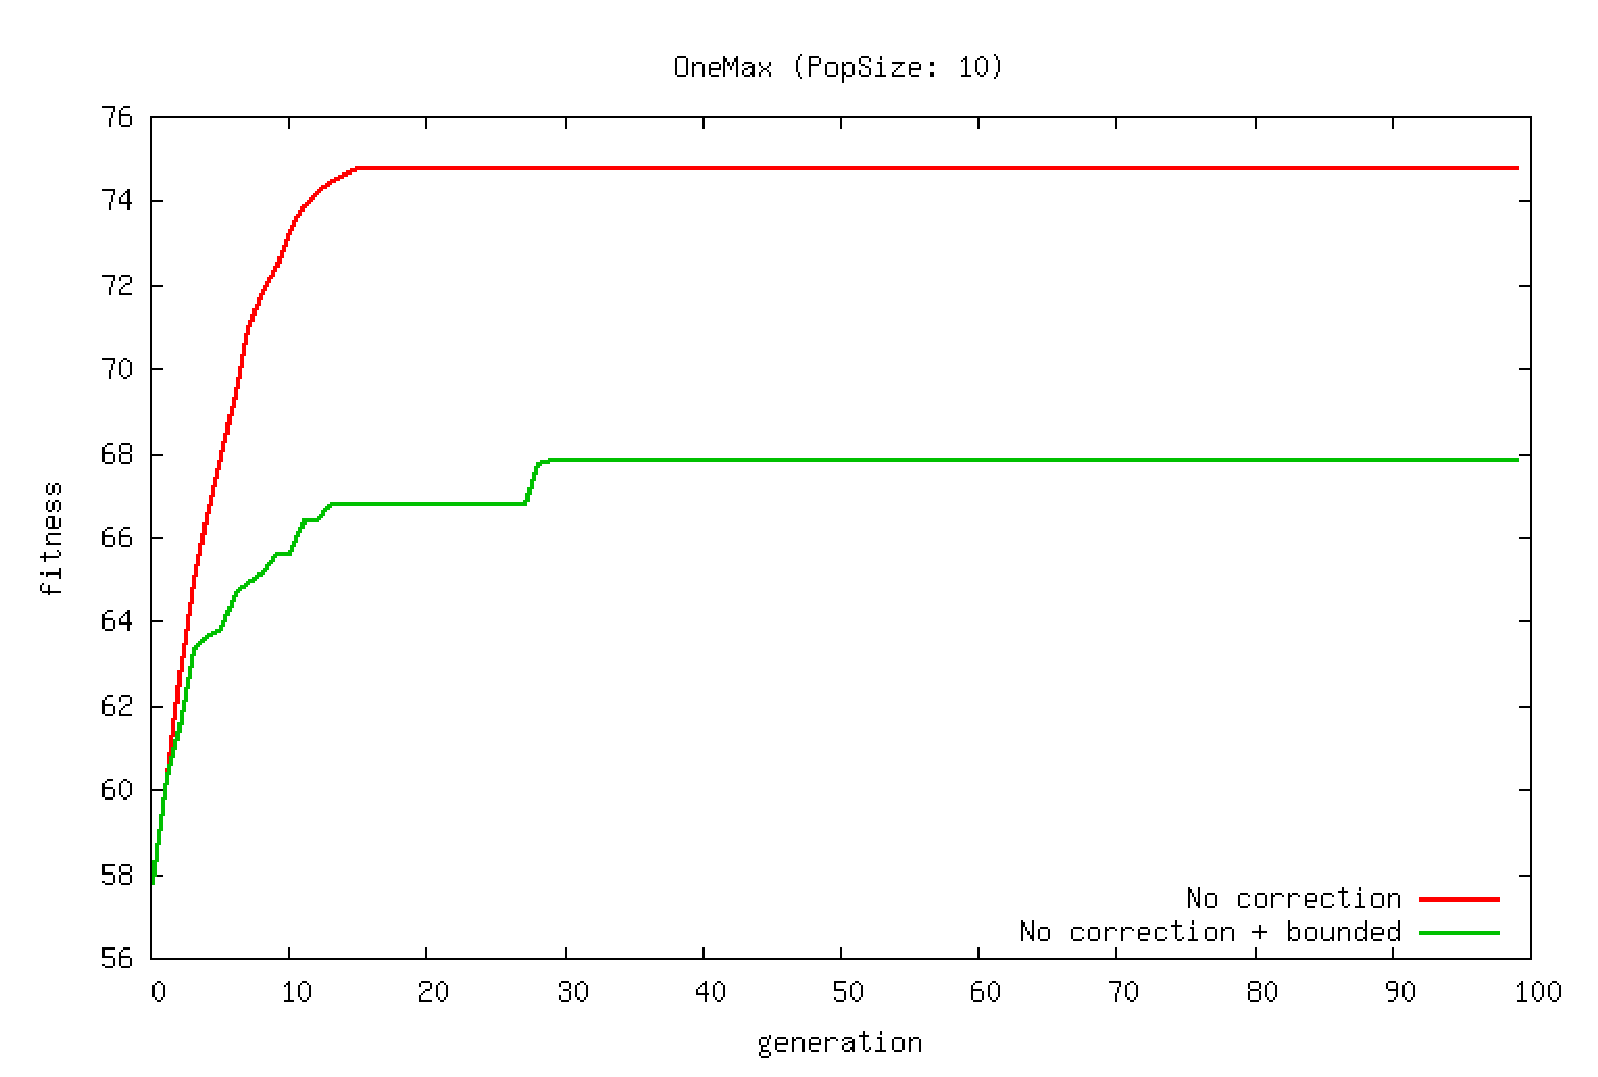
\includegraphics[scale=0.35]{graph_onemax_no_correction_bounded_fitness0.eps}
%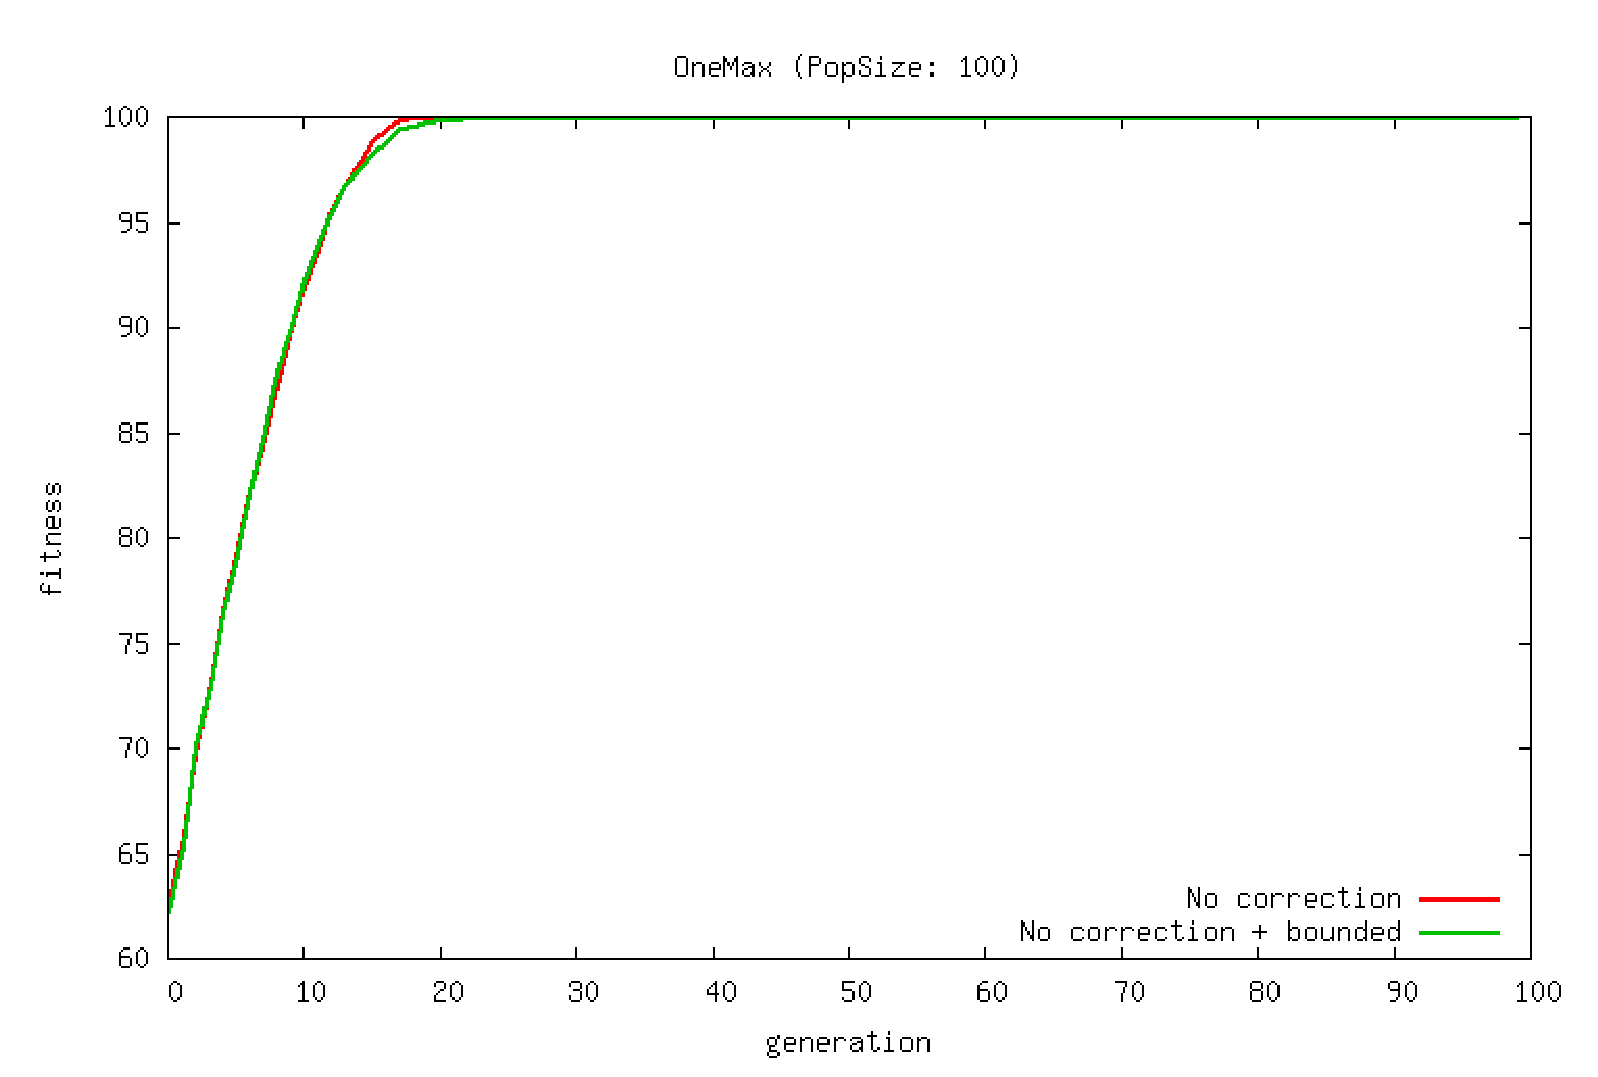
\includegraphics[scale=0.35]{graph_onemax_no_correction_bounded_fitness1.eps}
%\mycaption{With boundary check the diversity is held at a constant level}
%\label{bounded_2}
%\end{figure}

%\begin{figure}[H]
%\hspace{-0.5in}
%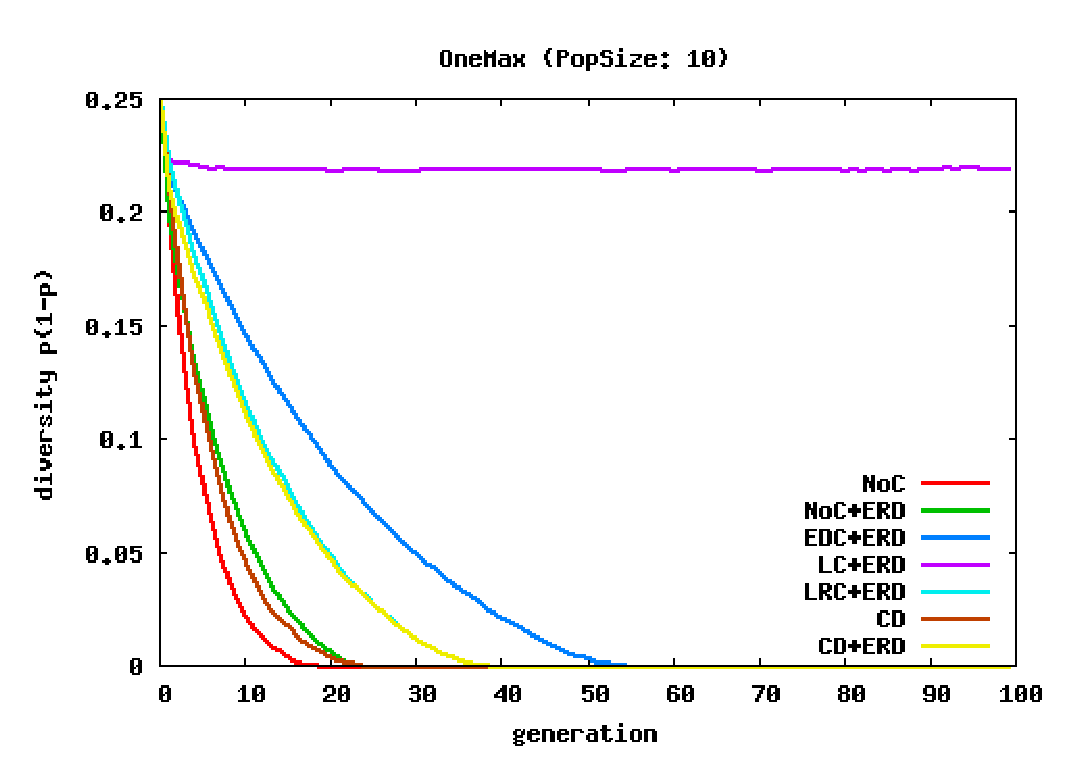
\includegraphics[scale=0.5]{graphs/graph_onemax1161008942/graph_onemax000_diversity.eps}
%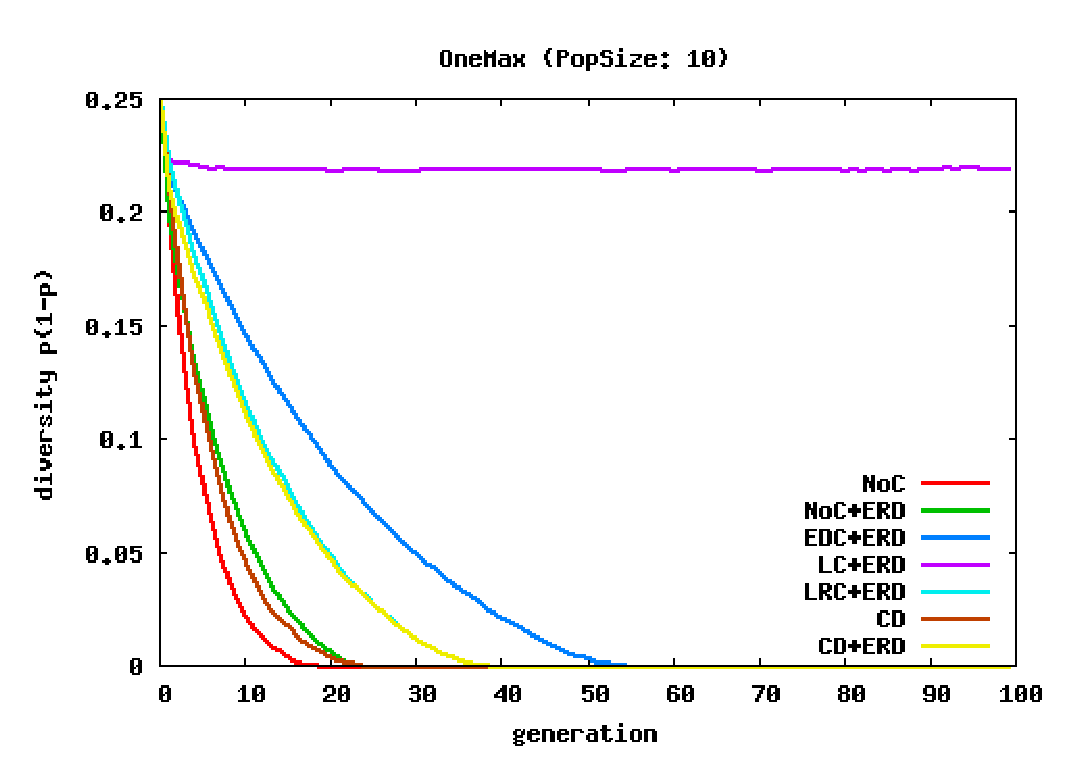
\includegraphics[scale=0.5]{graphs/graph_onemax1161008942/graph_onemax000_diversity.eps}
%\mycaption{TEST}
%\label{bounded_3}
%\end{figure}

\subsection{Laplace Correction (LC)}	

\begin{wrapfigure}{r}[0cm]{5.5cm}
\vspace{-0.7in}
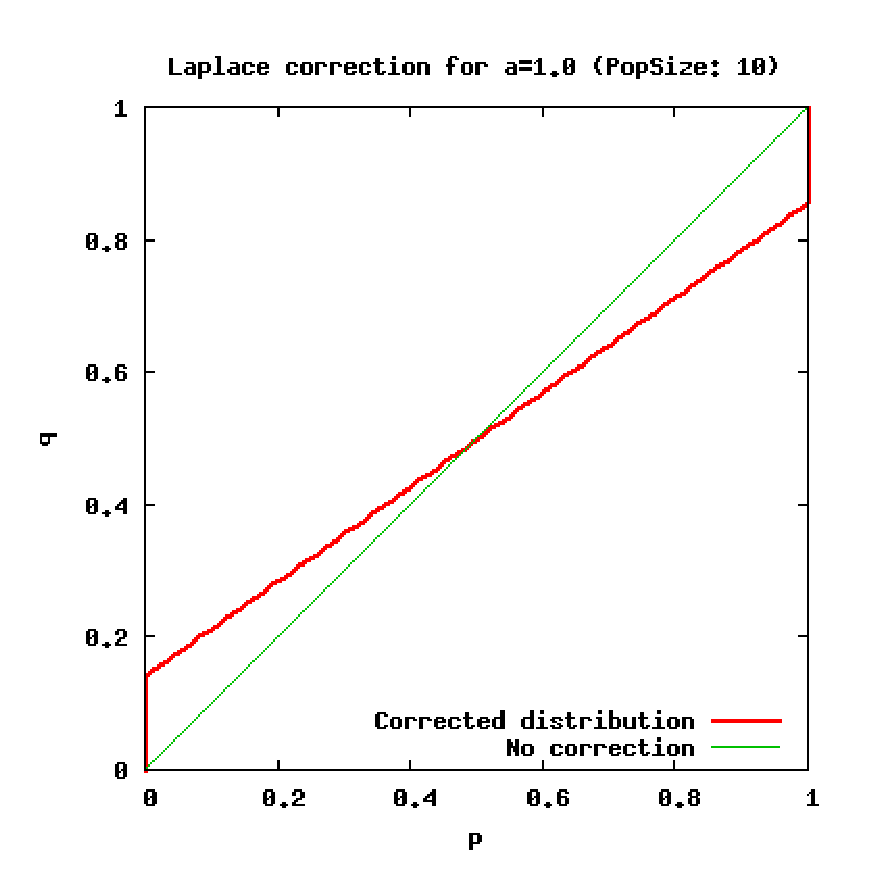
\includegraphics[scale=0.4]{graph_LC1_correction.eps}
\mycaption{Correction graph for Laplace Correction}
\label{lc_correction_1}
\end{wrapfigure}

Laplace correction is more or less the standard in connection with UMDA \cite{LaplaceStandard}. It biases the resulting \(p\) towards \(\frac{1}{2}\) and ensures that components do not get stuck at \(p = 1.0\) or \(p = 0.0\). The general formula for Laplace correction for a component \(i\) is to divide the number of '1's in the selected population plus \(\alpha\) by the size of the selected population plus \(2\alpha\):
\begin{equation}
p_{i} = \frac{k_{i} + \alpha}{N + 2\alpha}
\end{equation}

Unfortunately the optimal value for \(\alpha\) depends on the type of the problem and the problem parameters. While we have approximately \(\alpha = 0.03\) as the optimal value for the OneMax problem we have approximately \(\alpha = 0.15\) as the optimal value with the Plateau problem in figure~(\ref{laplace_alpha_1}) and the NK problem in figure~(\ref{laplace_alpha_2}). In addition there is always the trade-off between convergence speed and fitness for some problems. If we set \(\alpha\) very low we have a chance to get out of uniformity of a component but a low convergence speed. If we use higher values for \(\alpha\) we get faster to the optimal solution but are no longer able to keep good solutions.

\begin{figure}[H]
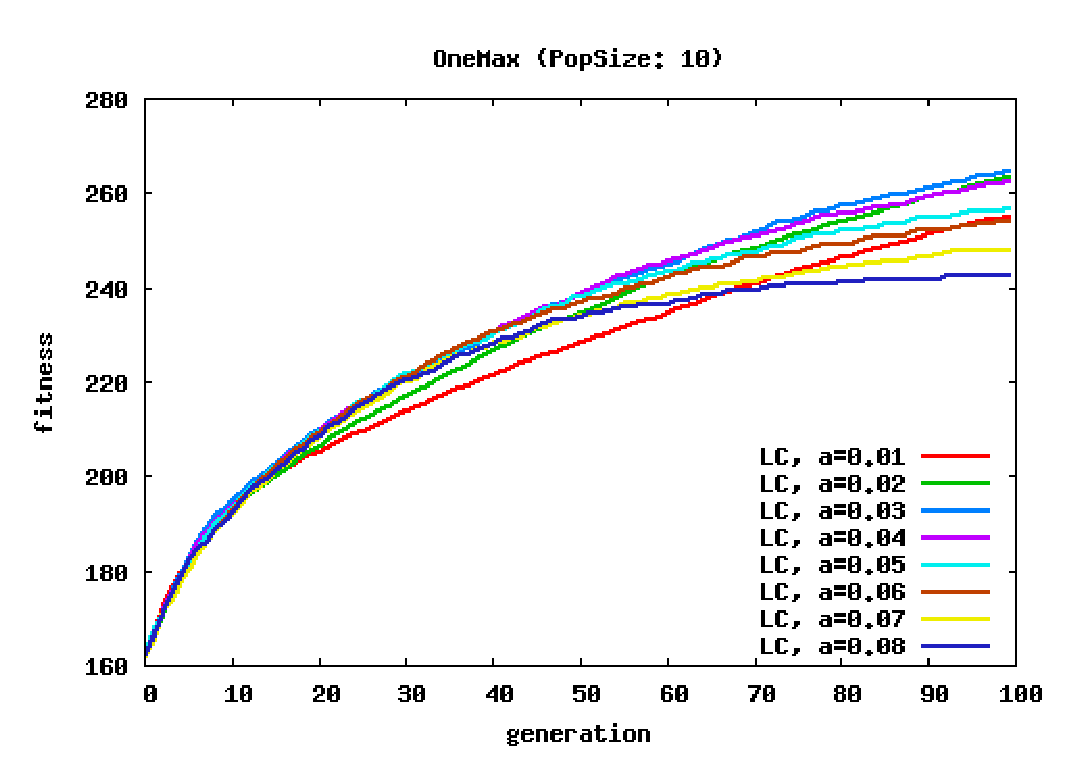
\includegraphics[scale=0.4]{graphs/graph_onemax1162151659/graph_onemax000_fitness.eps}
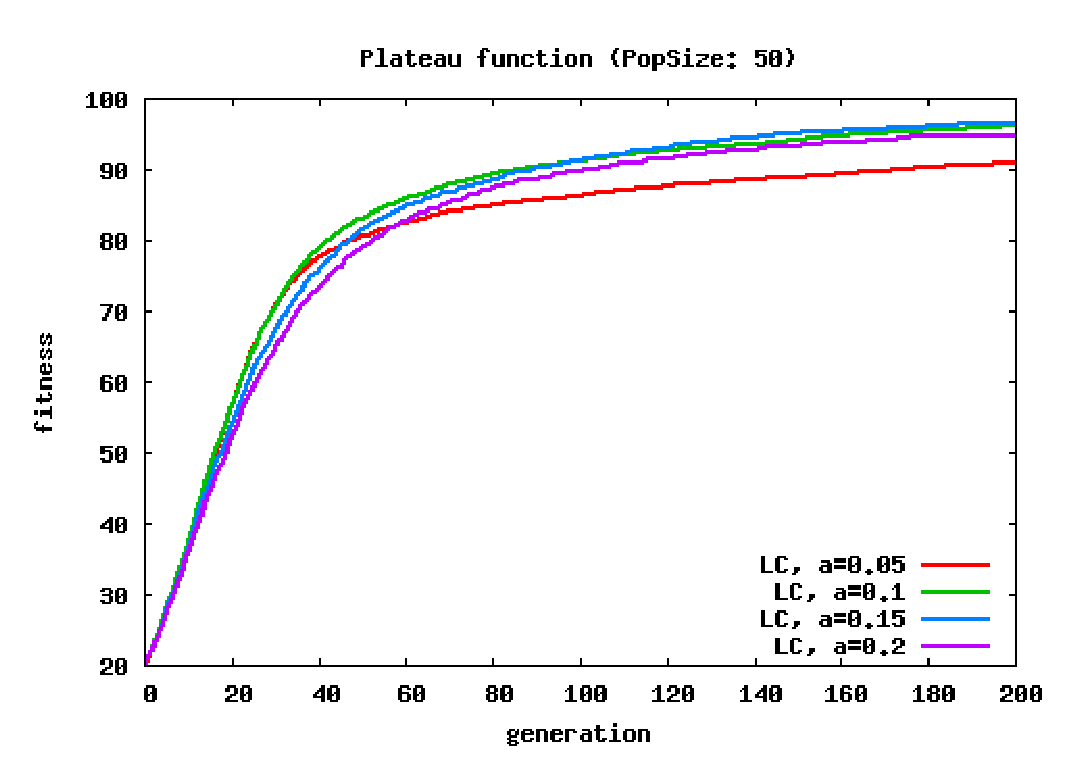
\includegraphics[scale=0.4]{graphs/graph_plateau1162152446/graph_plateau000_fitness.eps}
\mycaption{\(\alpha\) influences the effectiveness of Laplace correction but is problem-dependent}
\label{laplace_alpha_1}
\end{figure}

\begin{figure}[H]
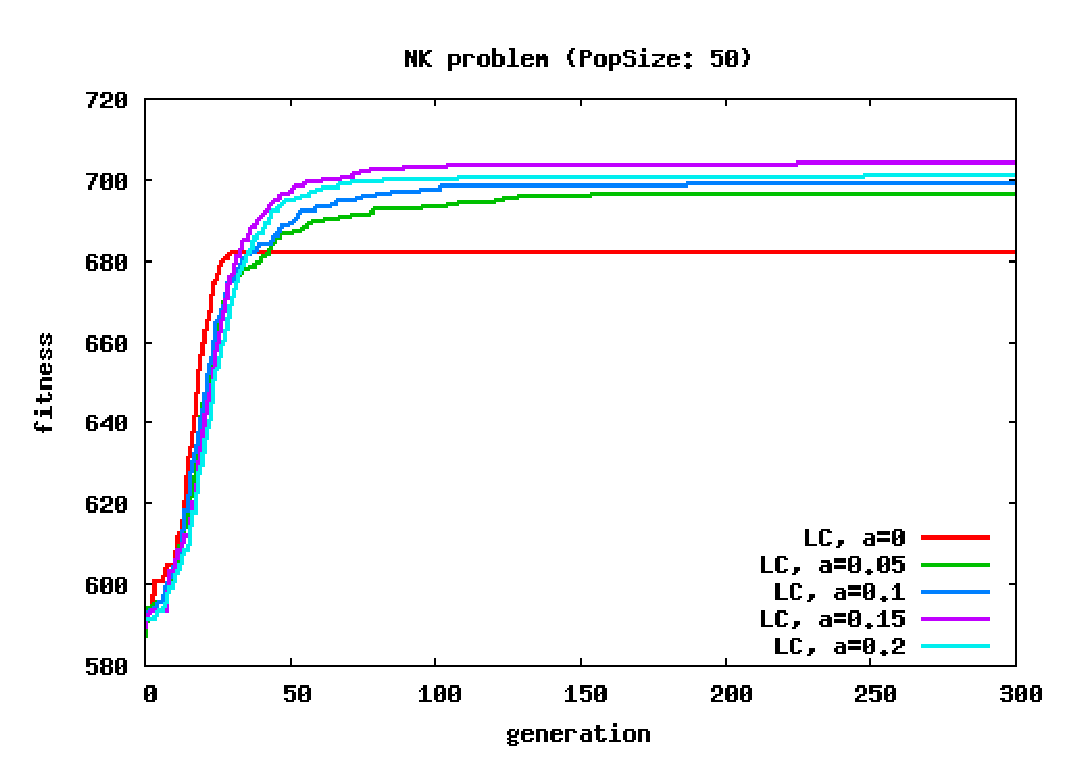
\includegraphics[scale=0.4]{graphs/graph_nk1162146485/graph_nk000_fitness.eps}
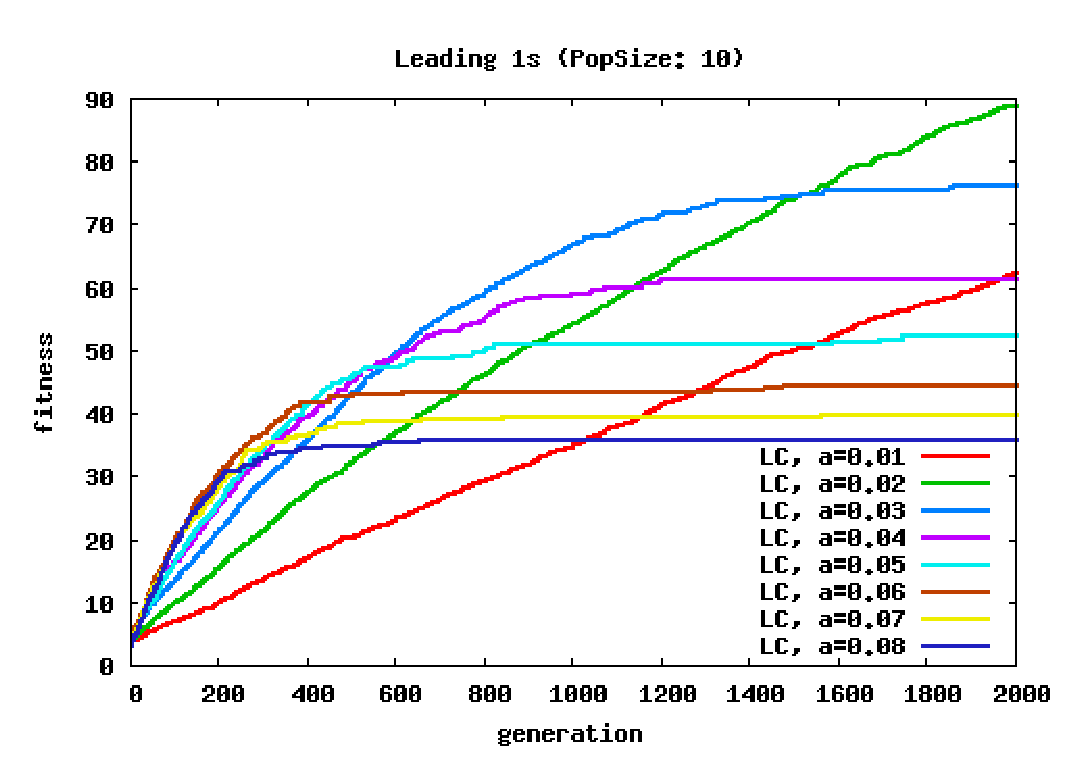
\includegraphics[scale=0.4]{graphs/graph_leading1162147298/graph_leading000_fitness.eps}
\mycaption{\(\alpha\) influences the effectiveness of Laplace correction but is problem-dependent}
\label{laplace_alpha_2}
\end{figure}


%\subsection{Laplace Remember Correction (LRC)}

%Another option is to include the distribution vector of the previous generation. We will replace \(\alpha\) in the numerator with \(\tilde{\alpha} = \alpha p_{t;i}\) where \(p_{t+1}\) denotes the new and \(p_{t}\) denotes the old distribution vector:

%\[
%p_{t+1;i} = \frac{k_{i} + \alpha p_{t;i}}{M + 2 \alpha}
%\]
%Contrary to Laplace Correction we have here of course no automatic boundary check as with a constant \(\alpha\) in the numerator.\\
%We will now compare this method with Laplace with \(\alpha = 1.0\) (other values of \(\alpha\) simply in- or decrease the constant level of variance). Looking at the variance on a flat fitness landscape, we can clearly see that using the previous distribution vector \(p\) as \(\alpha\) does not prevent diversity loss. TODO
%TODO

%\begin{figure}[H]
%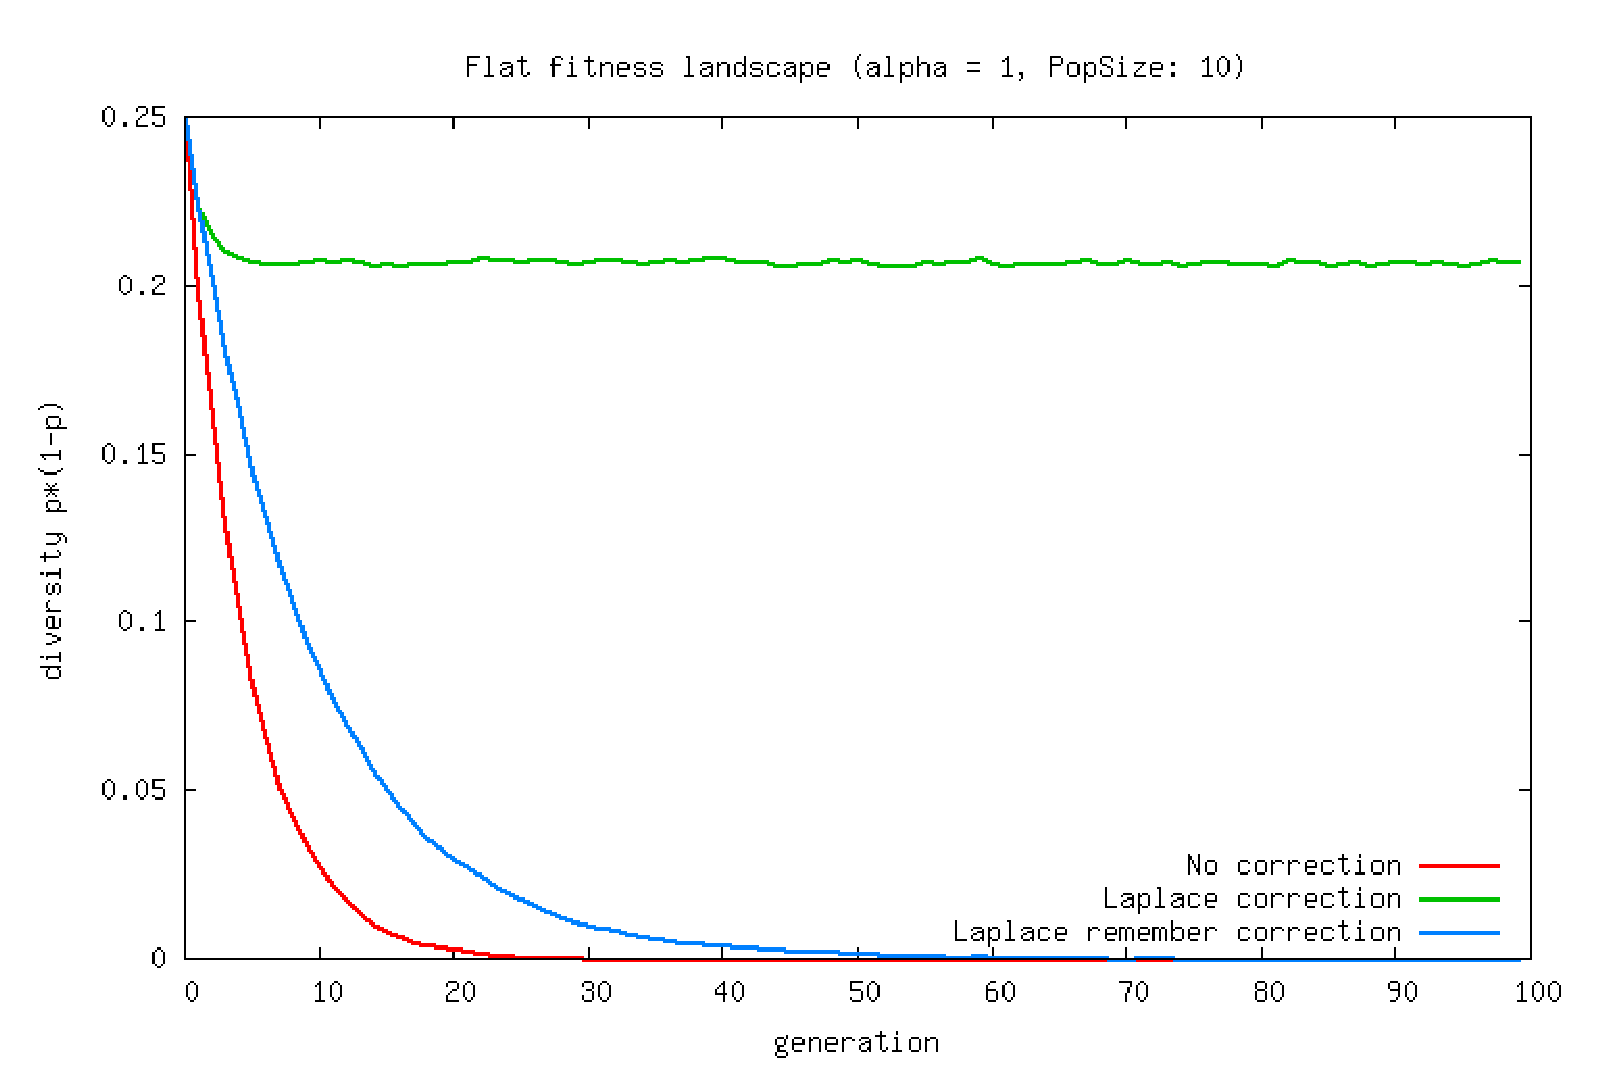
\includegraphics[scale=0.35]{graph_flat_laplace_diversity0.eps}
%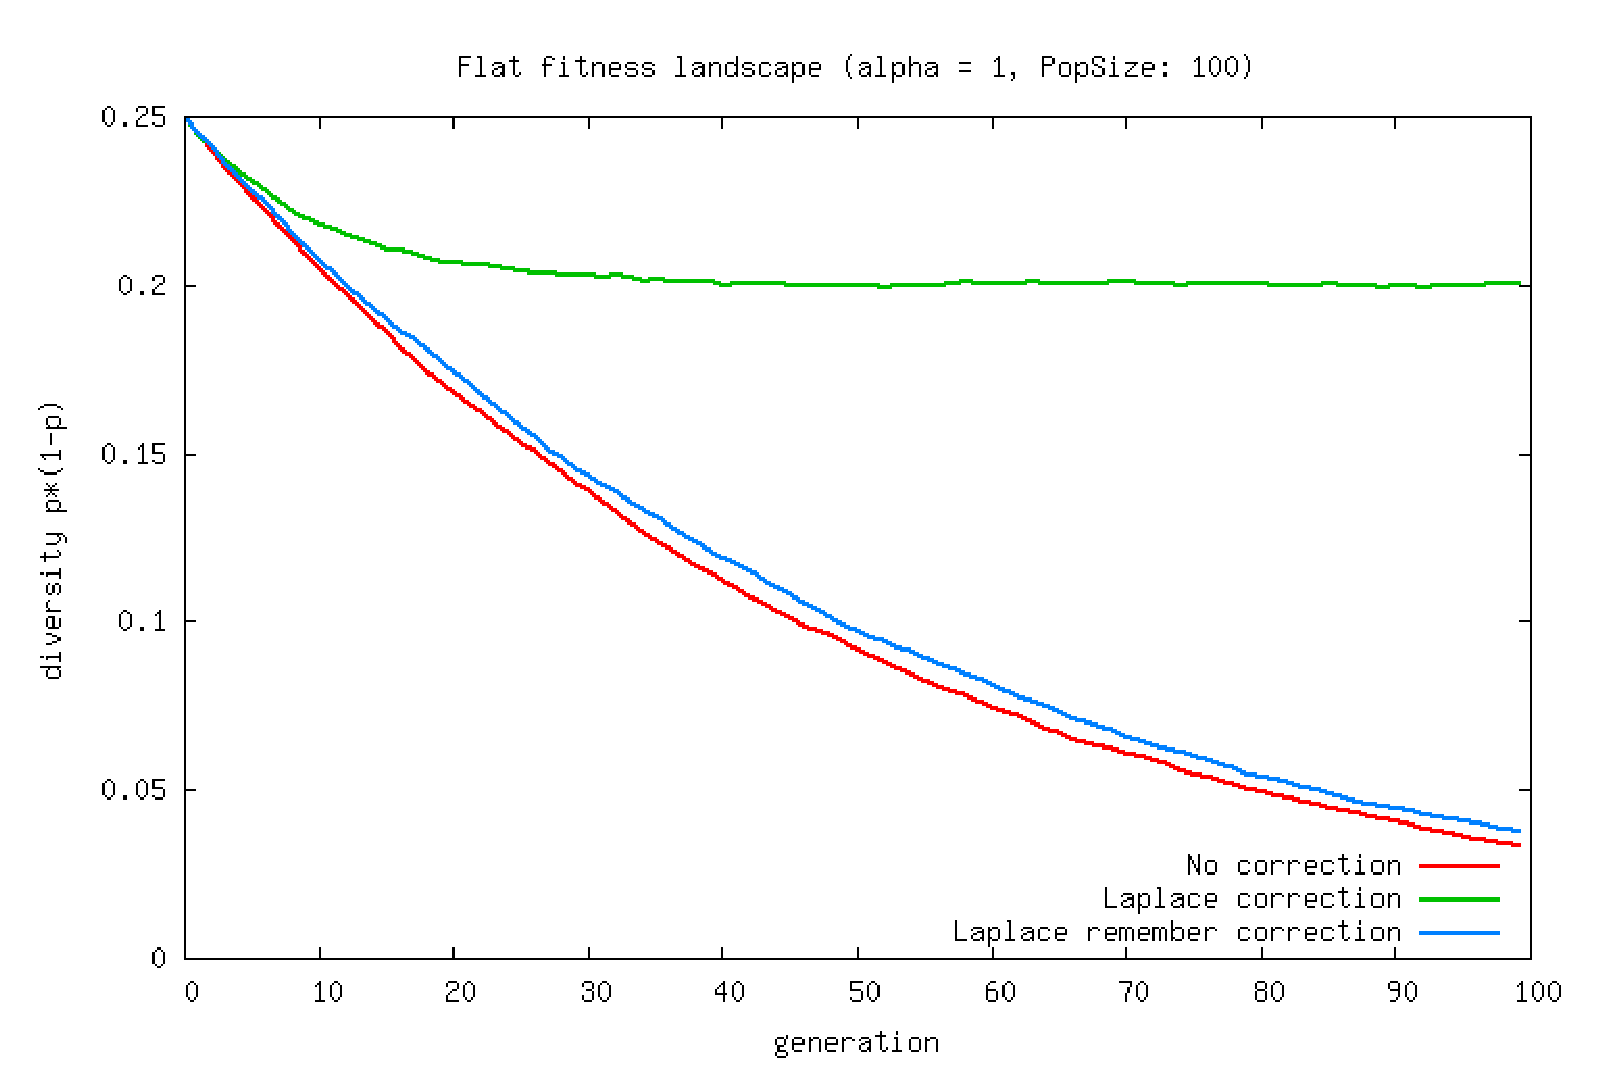
\includegraphics[scale=0.35]{graph_flat_laplace_diversity1.eps}
%\mycaption{TODO}
%\label{laplace_1}
%\end{figure}

%In the case of  ONEMAX: TODO
%- outperform laplace
%- higher population size - as usual - less advantage over no correction
%\begin{figure}[H]
%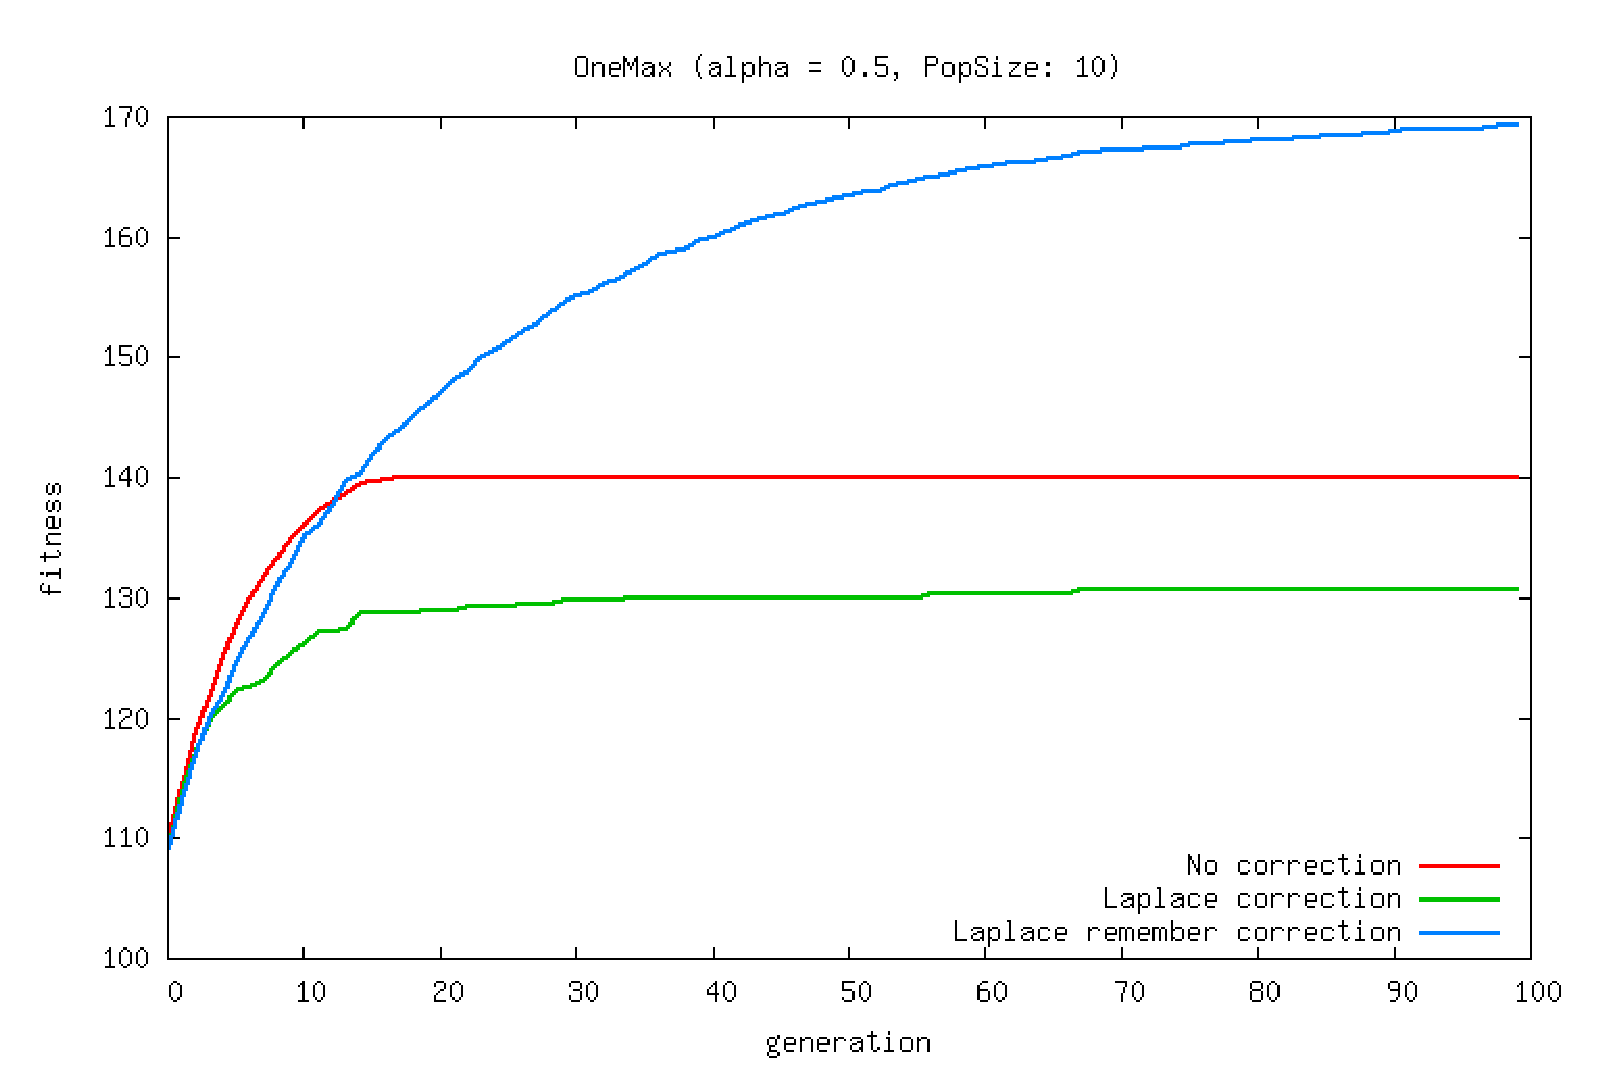
\includegraphics[scale=0.35]{graph_onemax_laplace_fitness0.eps}
%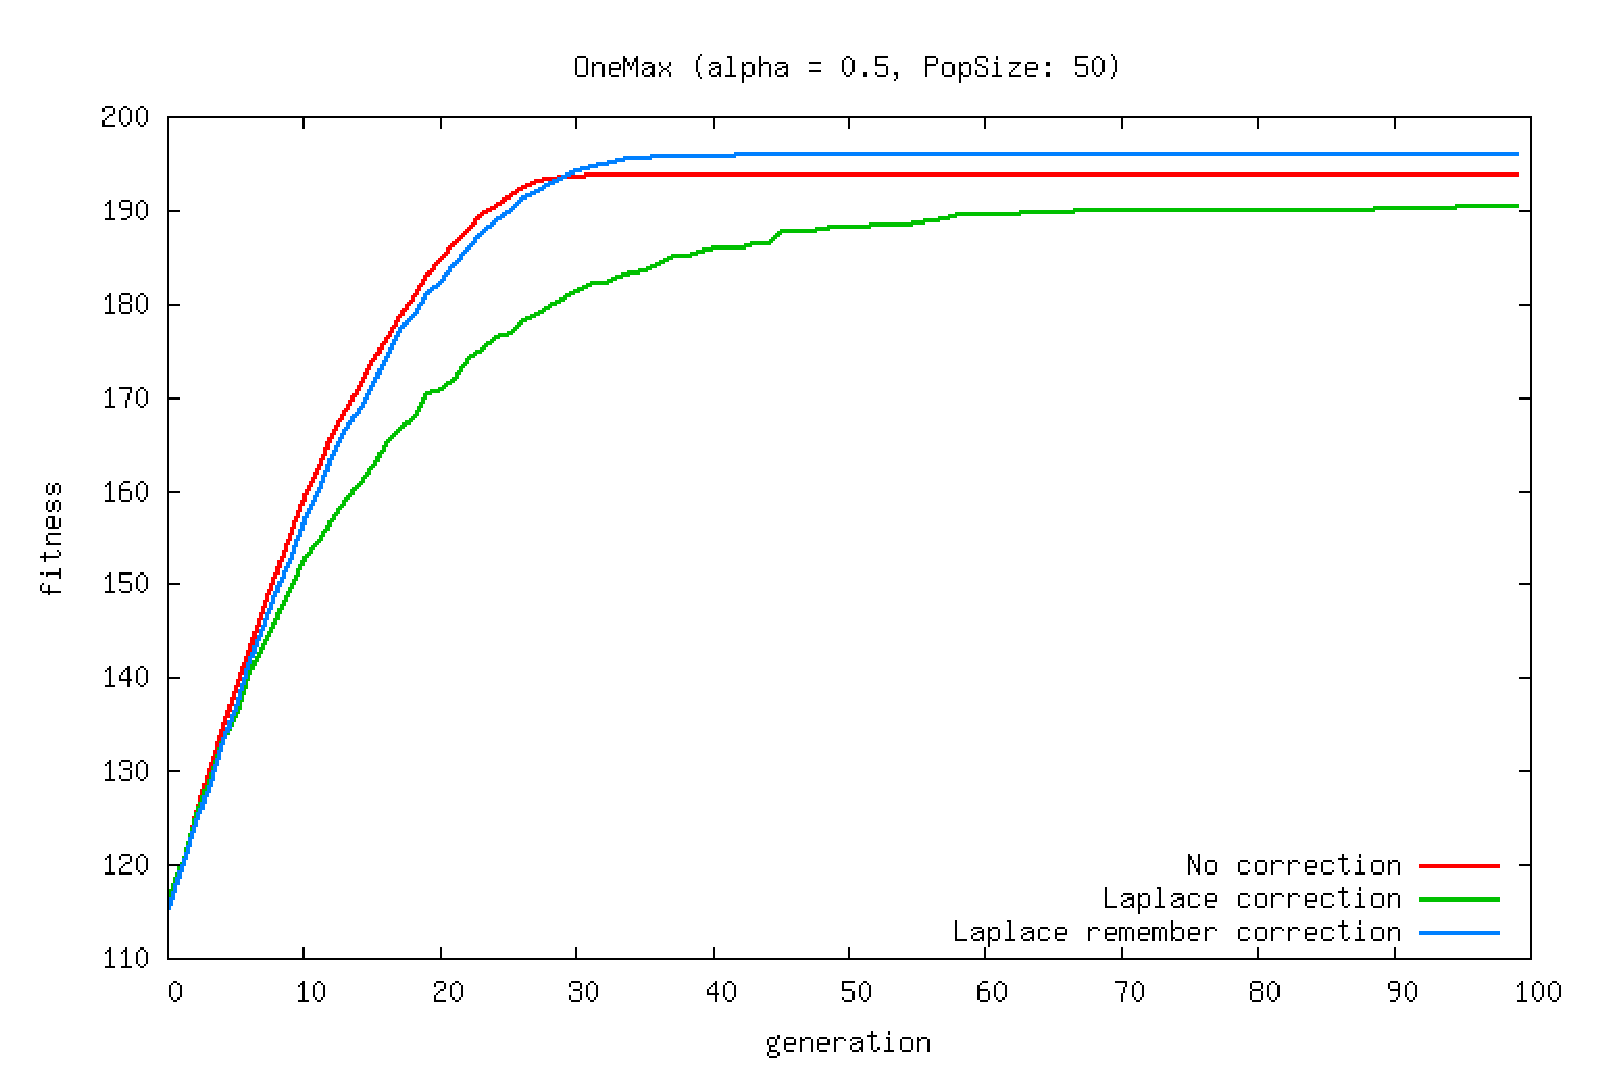
\includegraphics[scale=0.35]{graph_onemax_laplace_fitness1.eps}
%\mycaption{TODO}
%\label{laplace_2}
%\end{figure}
%TODO
%With this parameter settings and problem, higher values for \(\alpha\) will decrease the efficiency further:
%\begin{figure}[H]
%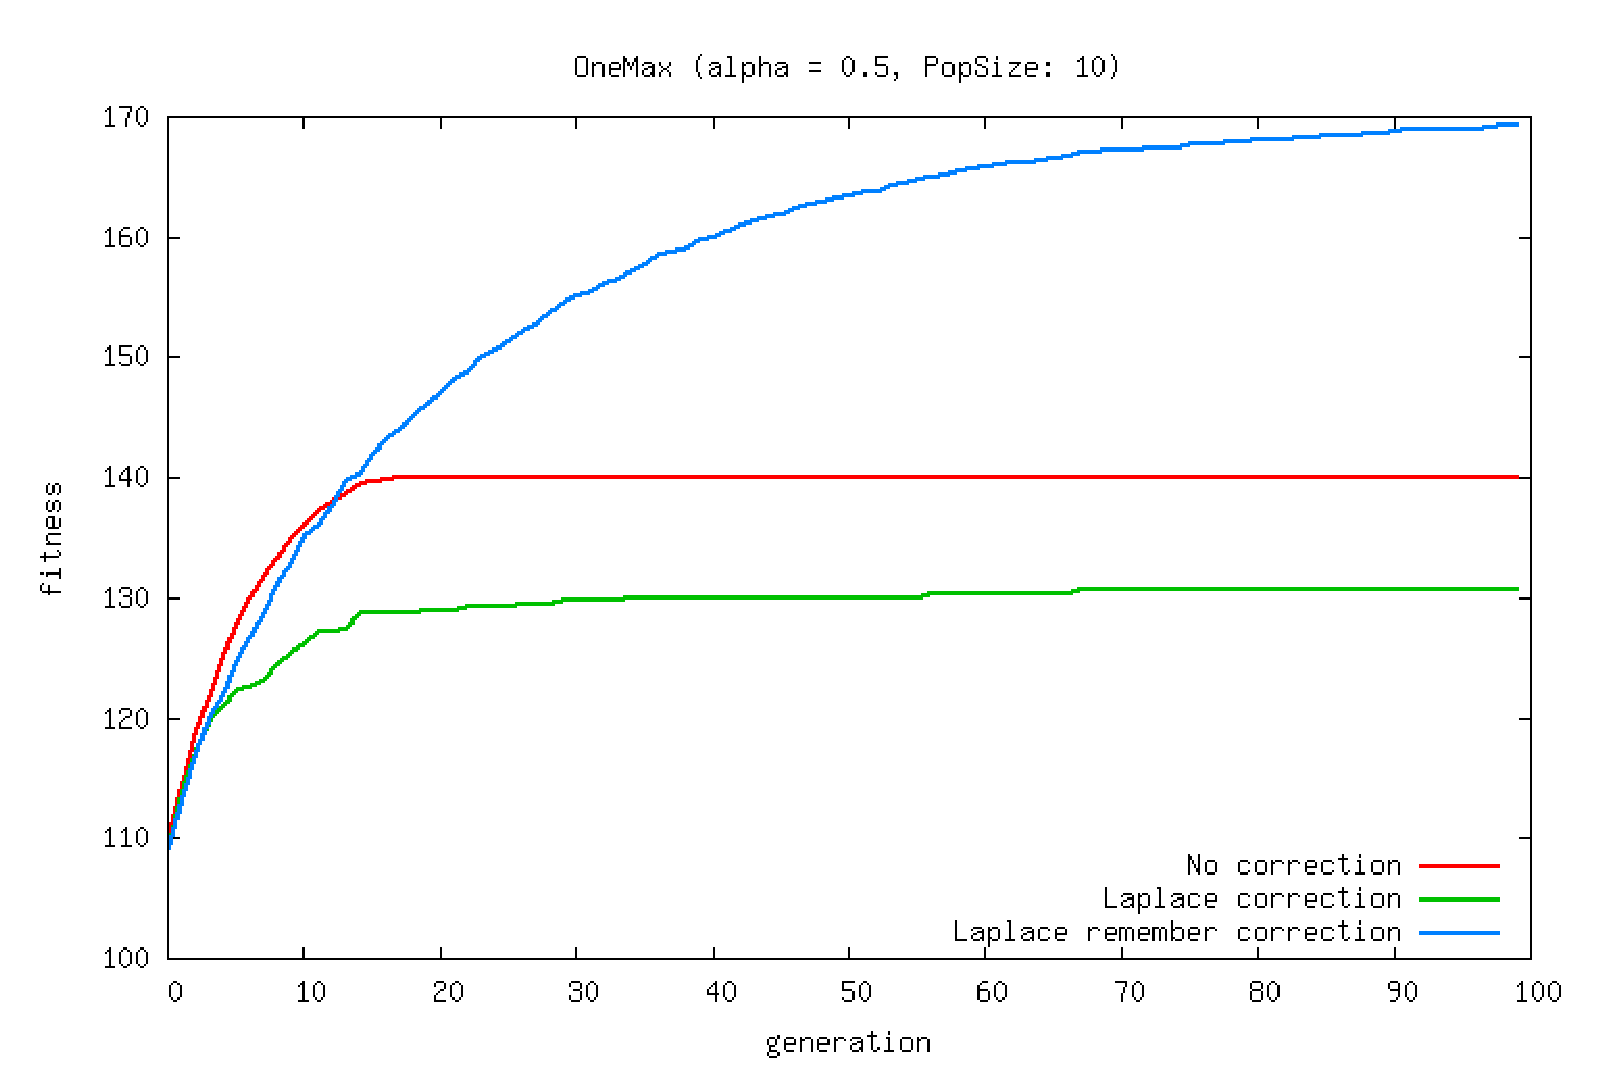
\includegraphics[scale=0.35]{graph_onemax_laplace_fitness0.eps}
%\mycaption{TODO}
%\label{laplace_3}
%\end{figure}

\newpage
\section{Comparison between the correction methods}

\subsection{Bounded vs. Laplace}

As we have discussed in the previous chapter, both Laplace Correction and Boundary Check does prevent \(p\) from getting to near the boundary values \(p = 0.0\) and \(p = 1.0\). In addition LC biases the resulting \(p\) to \(\frac{1}{2}\) due to the lower gradient. We can expect that Laplace Correction outperforms a simple Boundary Check in terms of variance on a flat fitness landscape, the question is if this bias is significant.\\
For the test we will look at configurations of \(\alpha\) and \(\beta\) that change \(p\) at the borders to the same values. Laplace Correction corrects \(p = 0\) to \(\frac{\alpha}{N + 2\alpha}\), Boundary Check corrects \(p = 0\) to \(\beta\), so in order to compare the behaviour at the borders we set \(\beta = \frac{\alpha}{N + 2\alpha}\). In figure~\ref{boundedvslaplace1} we have set \(\alpha = 0.1\) and \(beta = 0.02\) (for N = 5) and \(beta = 0.004\) (for N = 25). As expected we can see that LC does perform in both cases a little better than a simple Boundary Check but poorly compared to other correction methods.
\begin{figure}[H]
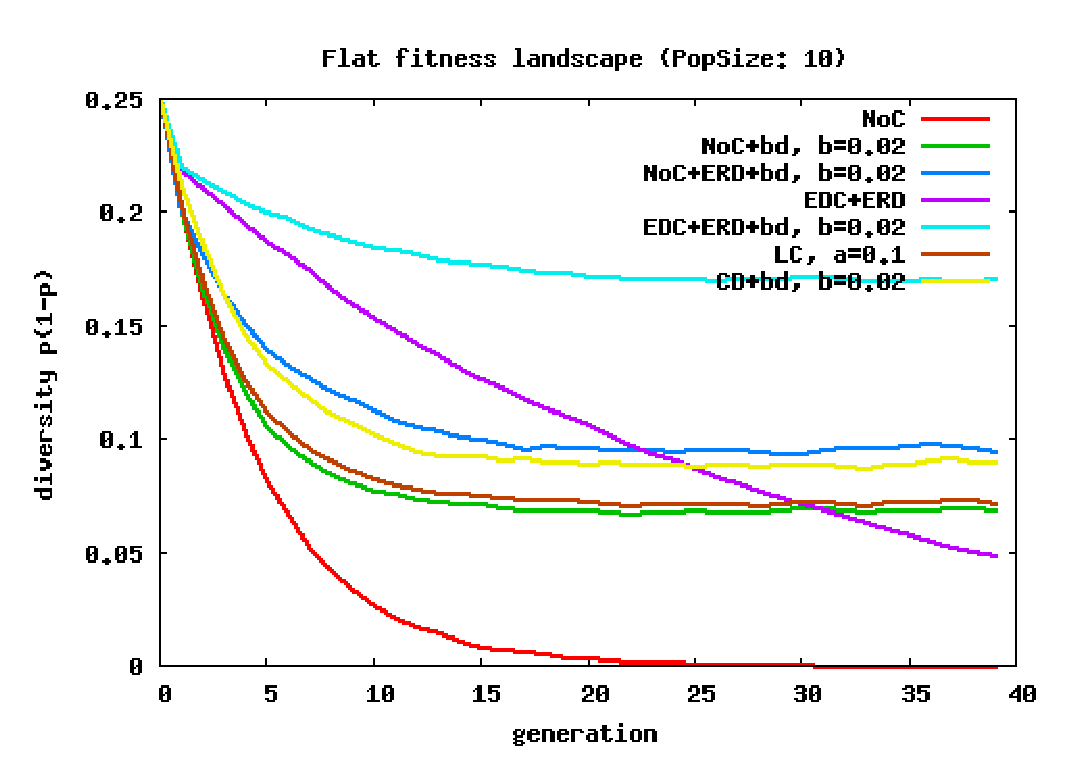
\includegraphics[scale=0.4]{graphs/graph_flat1162060937/graph_flat000_diversity.eps}
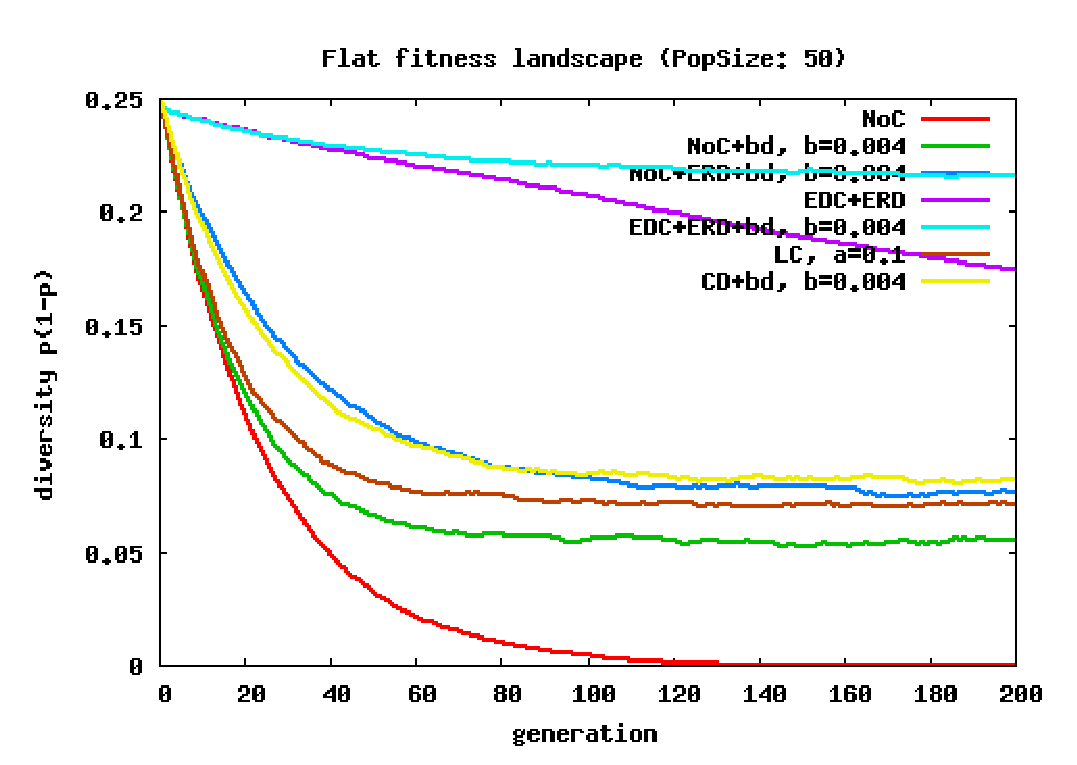
\includegraphics[scale=0.4]{graphs/graph_flat1162061548/graph_flat000_diversity.eps}
\mycaption{Comparison of diversity}
\label{boundedvslaplace1}
\end{figure}

When comparing the fitness with the OneMax problem (figure~\ref{boundedvslaplace2}) we see the same results, similar fitness and similar diversity. Exact Distriution Correction does not very well because it maintains a very high diversity which harms its fitness.
\begin{figure}[H]
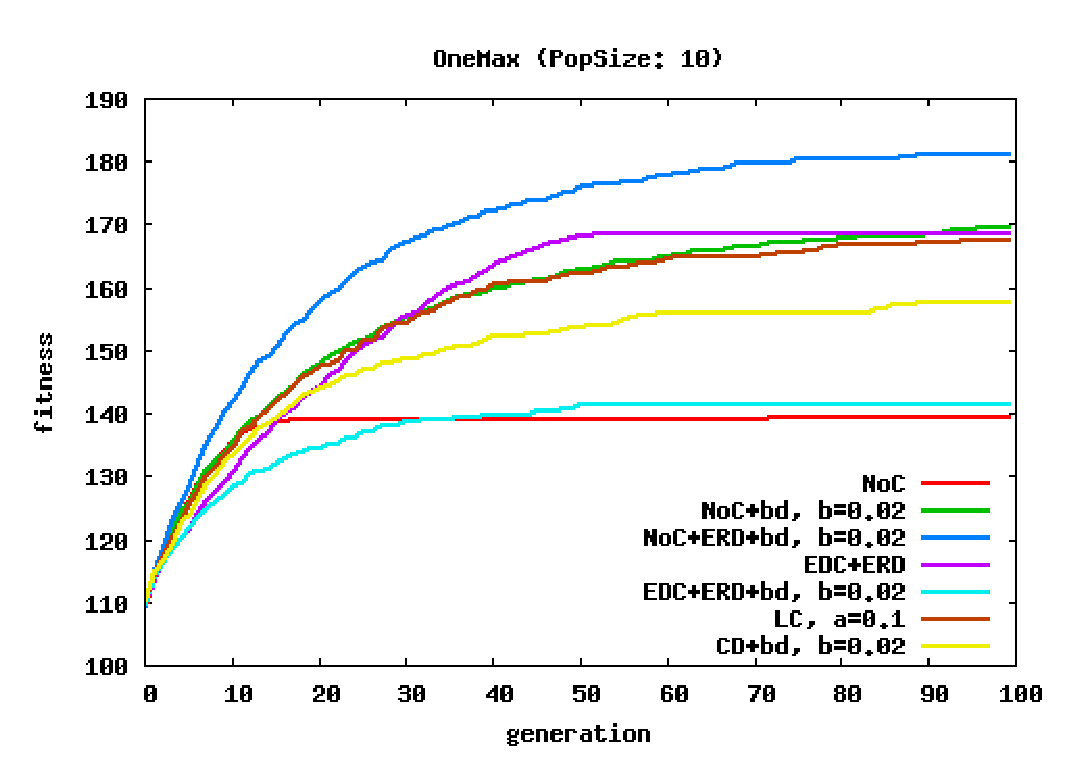
\includegraphics[scale=0.4]{graphs/graph_onemax1162062290/graph_onemax000_fitness.eps}
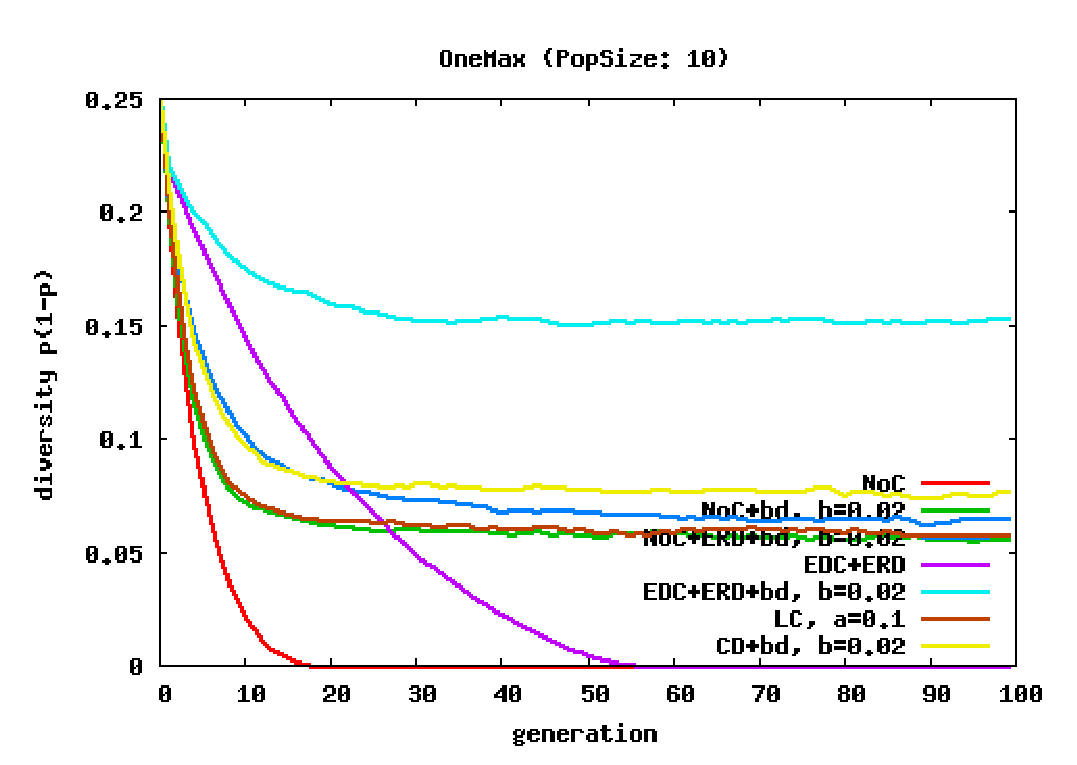
\includegraphics[scale=0.4]{graphs/graph_onemax1162062290/graph_onemax000_diversity.eps}
\mycaption{Comparison of fitness and diversity}
\label{boundedvslaplace2}
\end{figure}

At last a more difficult problem, a NK-landscape. In figure~\ref{boundedvslaplace3} we see again the same results.
\begin{figure}[H]
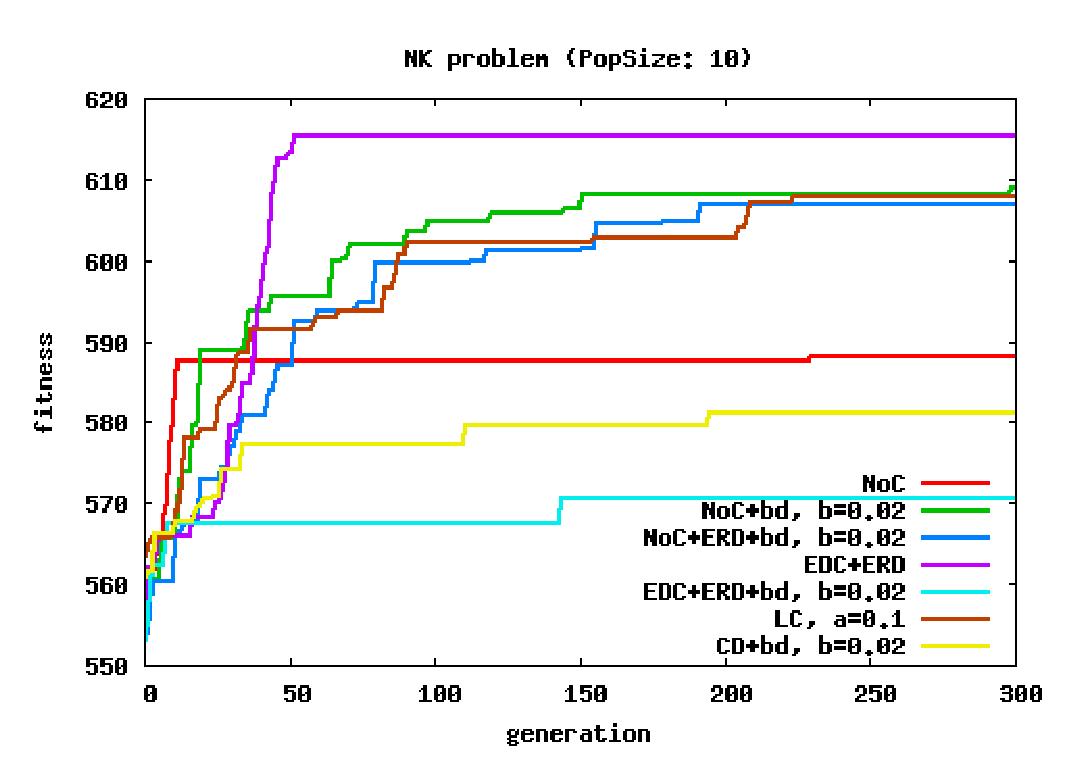
\includegraphics[scale=0.4]{graphs/graph_nk1162063368/graph_nk000_fitness.eps}
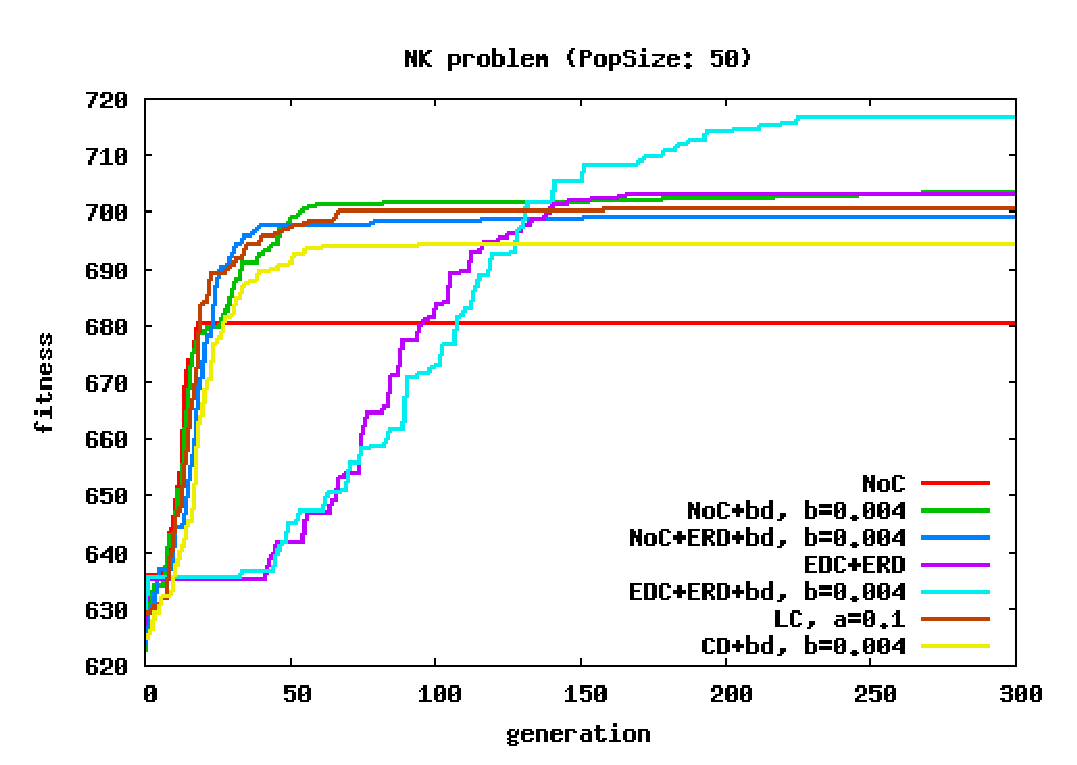
\includegraphics[scale=0.4]{graphs/graph_nk1162069892/graph_nk000_fitness.eps}
\mycaption{Comparison of fitness}
\label{boundedvslaplace3}
\end{figure}

TODO NK-Problem verfeinern, fuer mehr Werte, Testprogramm evtl aendern

% TODO ONEMAX
%'Corrected distribution + Laplace' is clearly worse than 'Laplace correction', the changes made to the distribution \(p\) (that we determined on base of the selected individuals) are too big in order to get useful results. As expected 'Laplace correction' itself does not score well, it converges at a significant lower fitness level.\\
%'Exact random distribution' seems to generally improve the convergence of methods using not the 'Laplace correction' while being indifferent or being even worse for the 'Laplace correction' itself.\\
%At least for the case of 'OneMax' and the given parameter configuration, 'Corrected distribution' in connection with 'Exact Random Distribution' seems to outperform all other methods.



%TODO test with small population sizes
%TODO verschiedene Werte fuer Alpha in ein Diagramm
%TODO
%With the tests we have shown that our 'Corrected distribution' algorithm does significantly reduce the diversity loss compared to an algorithm with no correction. Making sure that the algorithm does not stall in a component with \(p < \frac{1}{\tilde{n}}\) or \(p > 1 - \frac{1}{\tilde{n}}\) ("bounded") makes sure that the diversity does not drop to zero in the long run. 'Corrected distribution' does not outperform 'Laplace correction' as the latter always corrects any distribution towards \(p = 0.5\).

\subsection{Corrected Distribution vs. Exact Corrected Distribution}

%Convergence speed, 99 bits 0, 1 bit 1    
%exact
%max: *(1/selection) / generation
%random
%max:Abweichungen beschleunigen Konvergenz?

\begin{figure}[H]
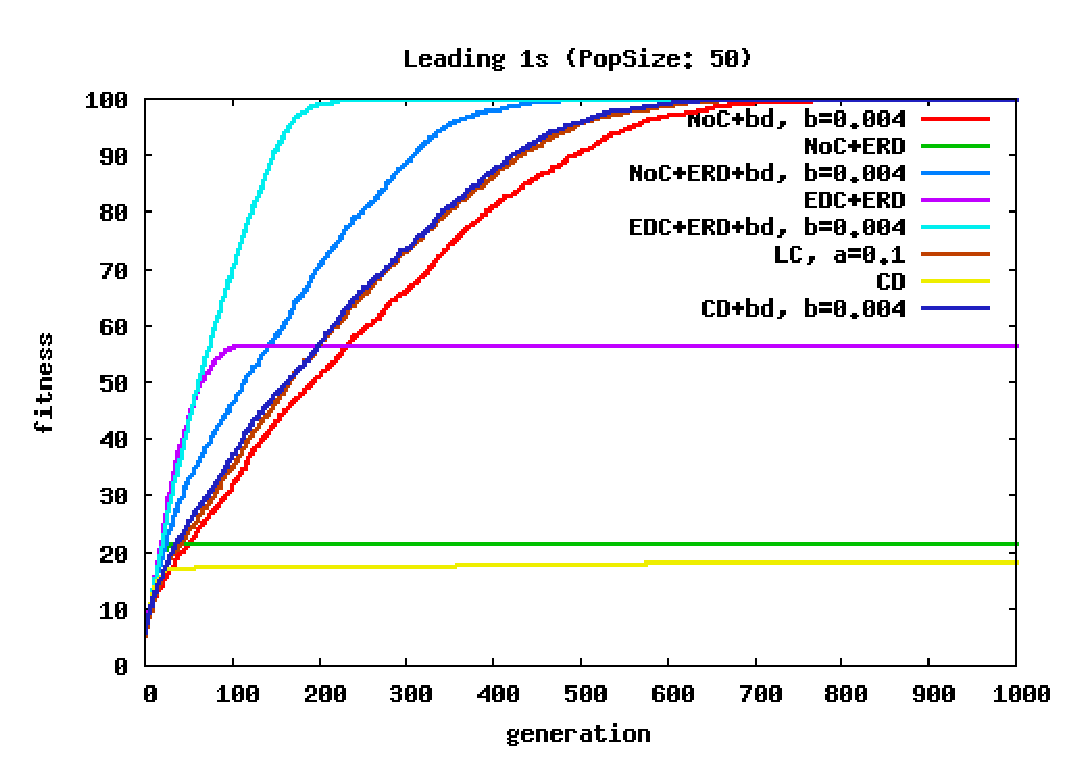
\includegraphics[scale=0.4]{graphs/graph_leading1162142917/graph_leading000_fitness.eps}
\mycaption{Comparison of fitness}
\label{erdvscd1}
\end{figure}

\begin{figure}[H]
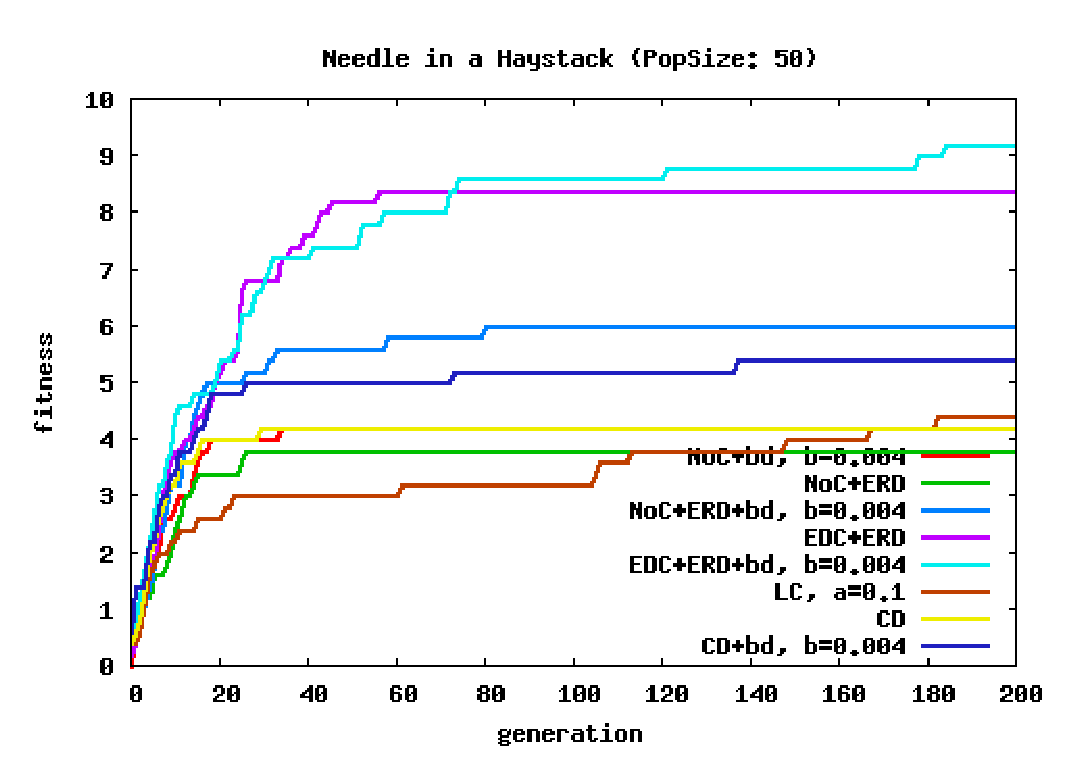
\includegraphics[scale=0.4]{graphs/graph_haystack1162144026/graph_haystack000_fitness.eps}
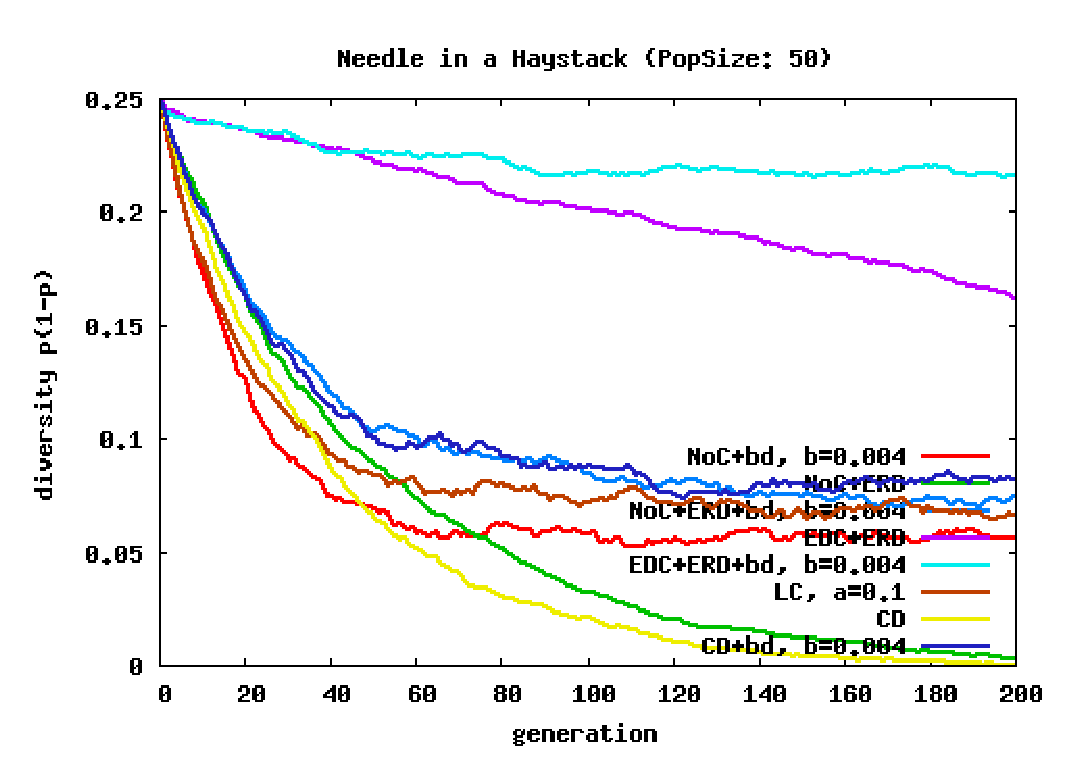
\includegraphics[scale=0.4]{graphs/graph_haystack1162144026/graph_haystack000_diversity.eps}
\mycaption{Comparison of fitness}
\label{erdvscd2}
\end{figure}


%\begin{figure}[H]
%\includegraphics[scale=0.4]{graphs/graph_onemax1162144026/graph_onemax000_fitness.eps}
%\mycaption{Comparison of fitness}
%\label{erdvscd3}
%\end{figure}


\begin{figure}[H]
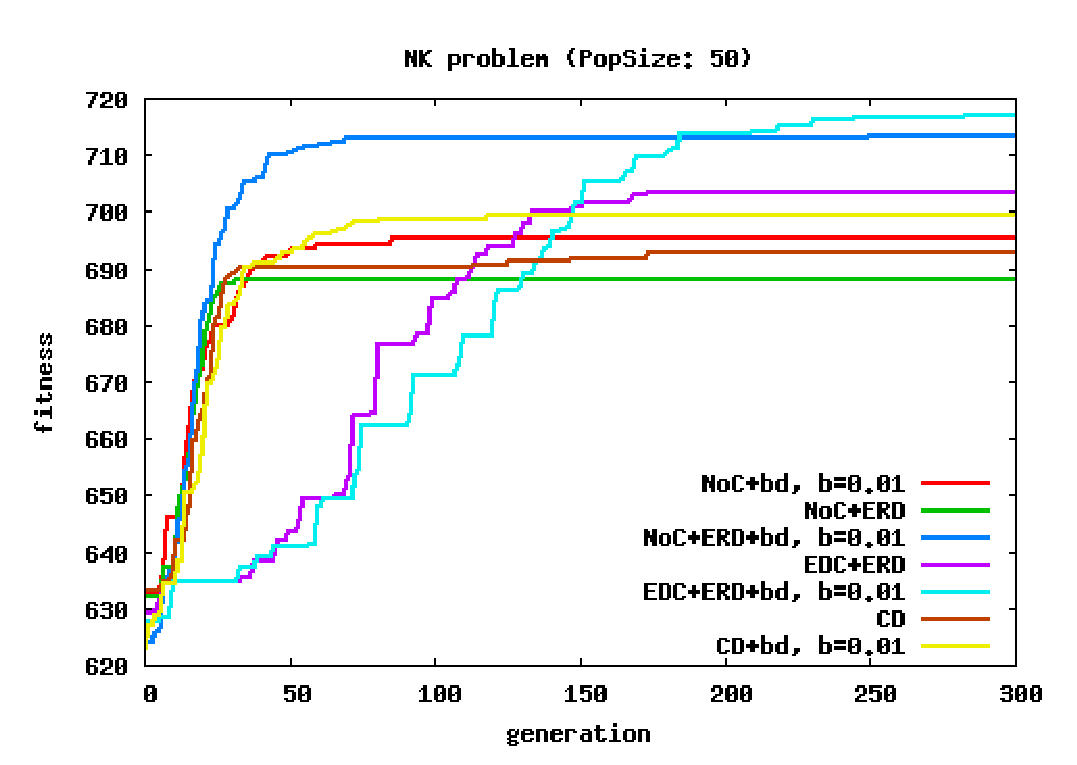
\includegraphics[scale=0.4]{graphs/graph_nk1162145639/graph_nk000_fitness.eps}
\mycaption{Comparison of fitness}
\label{erdvscd4}
\end{figure}

low population size -> bd

beste laplace
NC bounded
exact
exact+bounded
LC
DC
DC bounded


flat
onemax



\section{Fields of further research}

TODO

- |A| > 2
- Exact Diversity Correction - Rounding Error
- Proof of 1 - 1/M

According to \cite{Shapiro} the diversity loss of \(1 - \frac{1}{n}\) is independent of \(|A|\) and is valid for a whole class of so-called SML-EDAs, including UMDA, MIMIC, FDA or BOA. In this paper I have assumed that \(|A| = 2\), i.e. that a component can only take two different values. With values \(|A| > 2\) the proof has to be adapted from equation (5) on, depending on how one creates such a population. It also remains to be investigated how a similar correction of the diversity loss is possible with other methods than UMDA that fall into the category of the SML-EDAs. It is probable that the idea itself, i.e. determining the loss of variance due to sampling and calculating it backwards in order to correct the distribution \(p\), seems to be applicable to many different forms of SML-EDAs or even EDAs in general - assuming one can calculate the actual diversity loss.
\newpage

\begin{thebibliography}{99}
\bibitem{Shapiro} {\sc Shapiro, J.L.:}  \textit{Diversity loss in general estimation of distribution algorithms}, 2006.
\bibitem{Unknown1} {\sc Unkonwn:}  \textit{Source for |A| > 2 handling}.
\bibitem{LaplaceStandard} {\sc Unkonwn:}  \textit{Source for Laplace Standard UMDA}.
\bibitem{Muehlenbein} {\sc H. Muehlenbein and G. Paasz:}  \textit{From recombination of genes to the estimation of distributions: I. binary parameters.}, H.-M. Voigt, W. Ebeling, I. Rechenberg, and H.-P. Schwefel, editors, Parallel Problem Solving from Nature-PPSN IV, pages 178-187, Berlin, 1996. Springer. TODO
\bibitem{NKLandscape} {\sc Y. Gao and J. Culberson:}  \textit{An Analysis of Phase Transition in NK Landscapes}, http://www.cs.cmu.edu/afs/cs/project/jair/pub/volume17/gao02a.ps.Z
\bibitem{MitchelPotter} {\sc Potter, M.A.:}  \textit{NK-landscape problem generator}.
\bibitem{Rucksack} {\sc Unkonwn:}  \textit{Source for Rucksack UMDA representation}.


%http://www.comp.rgu.ac.uk/staff/ss/Publications/GECCO2005.pdf

\end{thebibliography}
\end{document}

